\chapter{Experimental Results}\label{ch:experimental-results}

At this point, I would like to note that all these executes had run in the computing grid of my university, the Technical University of Crete.
This grid consists of forty-four (44) nodes, each with four (4) CPUs.

At the beginning of each run, I was shuffling the input data.
I made this to create some randomness in my experiments.
For this reason, to have safe results and a sufficient statistical sample, I run thirty (30) times each experimental setup.
The results that came off from each case are the average of these runs.

The following plots show the final results.
There were a lot of failed attempts to reach them.
Each attempt cost four (4) days of continuous usage of the computing grid.

The numerical data that all the below plots are based are in Appendix~\ref{ch:detailed-experimental-results}.


\section{Models and Datasets}\label{sec:models-and-datasets}

\subsection{Classification problem}\label{subsec:classification-problem}

Looking into this GitHub repository~\cite{cnn_rnn_repo} without the usage of CNNs, I concluded that the best setup is with one LSTM layer with 19 units.
Finally, we add a Dense layer with 39 units (as the number of classes) to predict the category of the crime.

I selected the \emph{MSE} function for calculating the error and the \emph{Adam SGD} optimizer.
I also selected the \emph{ReLU} activation function for the LSTM layers and the \emph{Softmax} for the Dense.

\newpage

Regarding the hyperparameters, again based on this repository~\cite{cnn_rnn_repo}, I have chose,
\begin{itemize}
    \item \textbf{Points look back:} $5$
    \item \textbf{Learning rate:} $0.005$
    \item \textbf{Maximum optimizer iterations:} $500$
    \item \textbf{Sample shuffling:} Yes
    \item \textbf{Adam's tolerance:} $\expnumber{1}{-08}$
    \item \textbf{Adam's epsilon:} $\expnumber{1}{-08}$
    \item \textbf{Adam's beta1:} $0.9$
    \item \textbf{Adam's beta2:} $0.99$
\end{itemize}

\begin{figure}[H]
    \centering
    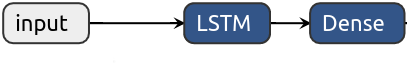
\includegraphics[scale=.3]{./images/impl/class-model.png}
    \caption{The structure of the DL Model for Classification purposes}
    \label{fig:dl_class_model}
\end{figure}

For this work, I selected the \textbf{San Francisco Crime Classification (SFCC)} dataset~\cite{sfc_dataset}.

This dataset contains incidents derived from SFPD Crime Incident Reporting system.
The data ranges from 1/1/2003 to 5/13/2015.

There are 9 variables:

\begin{itemize}
    \item Dates - timestamp of the crime incident
    \item Category - category of the crime incident.
    \item Descript - detailed description of the crime incident.
    \item DayOfWeek - the day of the week
    \item PdDistrict - name of the Police Department District
    \item Resolution - how the crime incident was resolved.
    \item Address - the approximate street address of the crime incident.
    \item X - Longitude.
    \item Y - Latitude
\end{itemize}

The dataset had totally 878,049 samples.
I split the data into training and testing samples with a ratio equivalent to 0.85.
In other words, the training samples were approximately 746,340 while the testing was approximately 131,700 samples.
The load that got each worker was equal.

The goal is predict the category of crime that occurred, given the time and location and the rest of variables.
The number of crime categories is $39$ which is the number of classes.

\subsection{Natural Language Processing problem}\label{subsec:natural-language-processing-problem}

The model was built to make sentiment analysis for as much as we have an NLP problem.
The input is sequences of words and the output is the case that this sequence is either positive or negative.
The structure of the model is represented below.

\begin{figure}[H]
    \centering
    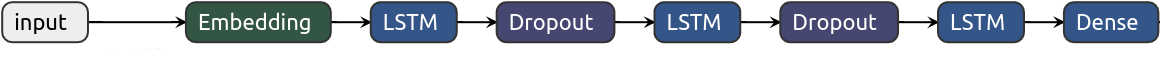
\includegraphics[scale=.3]{./images/impl/nlp-model.png}
    \caption{The structure of the DL Model for NLP purposes}
    \label{fig:dl_nlp_model}
\end{figure}

Here, we see that the first is the input layer.
Inside the layer, there is a built-in word embedding layer, which I implemented through the Python and the sklearn library.
A word embedding is a class of approaches for representing words and documents using a dense vector representation.
It is an enhancement over the traditional bag-of-word model encoding schemes where large sparse vectors used to describe each word or to score each word within a vector to represent a complete vocabulary.
These representations were sparse because the vocabularies were enormous and a given word or document would be represented by a large vector comprised mostly of zero values.
Rather, in an embedding, words are represented by dense vectors where a vector represents the projection of the word into a continuous vector space.
The position of a word within the vector space is learned from the input text and is based on the words that surround the word when it is used.
The method of learning word embeddings from the text I chose was the \emph{word2vec} algorithm.

Based on this article~\cite{rushabhwadkar_2019} and after a bunch of runs of trying not to reduce the accuracy, I concluded that the best setup is a stacked LSTM with three (3) layers.
Both the first and the second layer has 256 units.
The third one has 128.
Finally, we add a Dense layer with 1 unit to help decide if the sequence has a positive or negative sentiment.

I selected the \emph{MSE} function for calculating the error and the \emph{Adam SGD} optimizer.
I also selected the \emph{ReLU} activation function for the LSTM layers and the \emph{Sigmoid} for the Dense.

\newpage

Regarding the hyperparameters, again based on this article~\cite{rushabhwadkar_2019}, I have chose,
\begin{itemize}
    \item \textbf{Words look back:} $30$
    \item \textbf{Learning rate:} $0.005$
    \item \textbf{Maximum optimizer iterations:} $1000$
    \item \textbf{Dropout rate:} $0.2$
    \item \textbf{Sample shuffling:} Yes
    \item \textbf{Adam's tolerance:} $\expnumber{1}{-08}$
    \item \textbf{Adam's epsilon:} $\expnumber{1}{-08}$
    \item \textbf{Adam's beta1:} $0.9$
    \item \textbf{Adam's beta2:} $0.99$
\end{itemize}

For this work, I selected the \textbf{Amazon Fine Food Reviews (AFFR)} dataset~\cite{amazon_dataset}.

This dataset consists of reviews of fine foods from Amazon.
The data span a period of more than ten (10) years, including all $500,000$ reviews up to October 2012.
Reviews include product and user information, ratings, and a plain text review.
It also includes reviews from all other Amazon categories.

In detail, the dataset includes:

\begin{itemize}
    \item Reviews from October 1999 to October 2012
    \item 568,454 reviews
    \item 256,059 users
    \item 74,258 products
    \item 260 users with $>$ 50 reviews

\end{itemize}

From all the above details, I cared only for the reviews.
Hence, my dataset had 568,545 samples.
I split the data into training and testing samples with a ratio equivalent to 0.85.
In other words, the training samples were approximately 483,000 while the testing was approximately 85,200 samples.
The load that got each worker was equal.

\newpage

\section{Results}\label{sec:results}

In this section, I will present the results of this work.
I separated the results in two parts.

In the first part, I compare the two protocols using the same safe function.
This function is called \textbf{spherical cap} (Eq.~\ref{eq:equation36}) and is defined in section~\ref{sec:distributed-learning-using-fgm-protocol}.
I chose this function because in the next subsection I will prove that is better than the other (simple norm).

In the second part, I compare the two safe functions using -this time- the same protocol.
I chose the FGM protocol.

I have divided the experiments into three (3) subgroups.
In each case, the accuracy, the number of rounds, and the network traffic are compared each time with a different variable.
The first group is regarding the \textbf{threshold} ($T$), the second is regarding the \textbf{batch size} ($b$),
while the third one is regarding the \textbf{number of workers} ($k$).

\subsection{Protocols comparison}\label{subsec:protocols-comparison}

Firstly, I would like to note the accuracy that the model had when I trained it in a centralized way.
A centralized way is when only one worker undertakes the learning process.
To attain a logical comparison of the accuracy, I consider that the maximum value that the model can achieve is via centralized training.

The model for classification purposes had $99.59\%$ while the  NLP one had $98.37\%$ accuracy.

In Figure~\ref{fig:sfcc-affr_1} A,B, we see the accuracy, the number of rounds and the traffic when the threshold changes.
It is reasonable that all of them decrease over the threshold increase because of the lack of communication.
It happens because the violation condition has relaxed.
This reduction of accuracy is not so notable as to make our model tolerant of less communication.
Besides, we observe that the absolute number of rounds is greater in the AFFR dataset than the other (Fig.~\ref{fig:sfcc-affr_1} C,D).
It arises not only from the nature of the problem but also the structure of the model.
The model for the AFFR dataset has two additional LSTM layers.
For this reason, the traffic is much more in NLP model training (Fig.~\ref{fig:sfcc-affr_1} E,F).
It is also notable that both curves about the number of rounds and traffic follow the same direction.

\begin{figure}[H]
    \centering
    \begin{subfigure}[b]{0.45\textwidth}
        \centering
        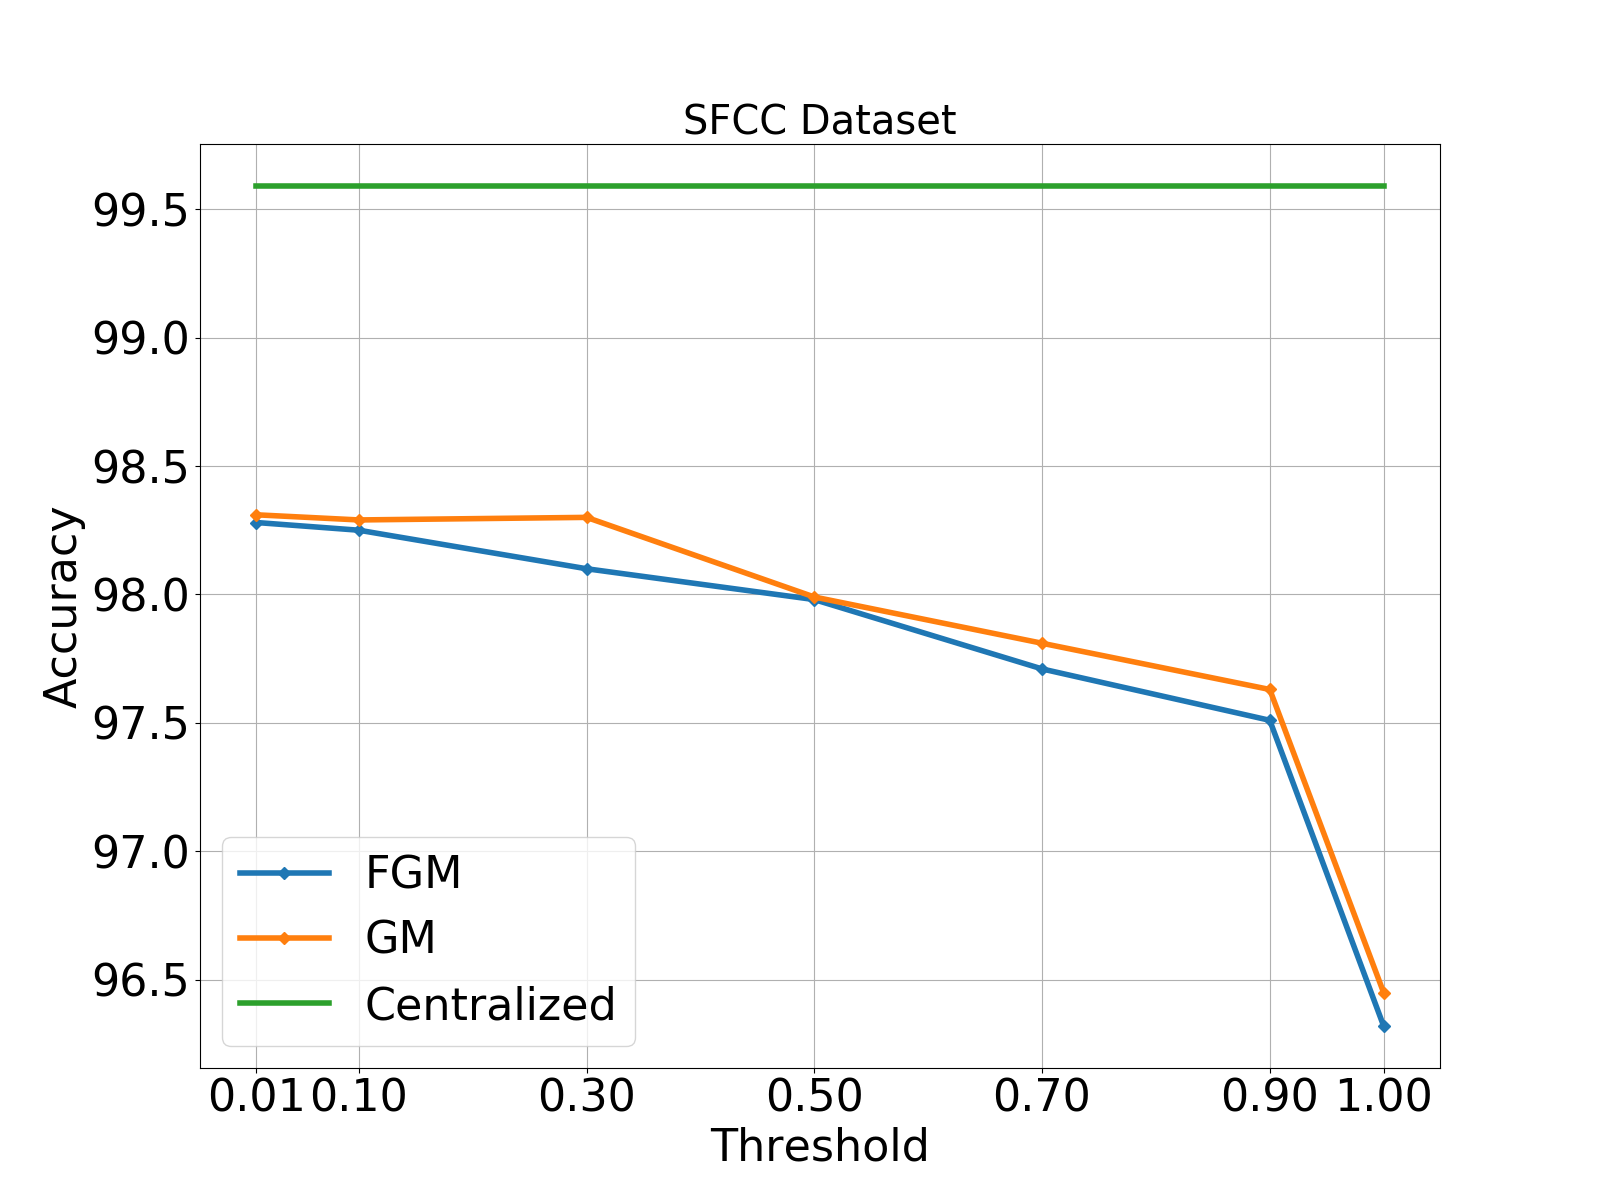
\includegraphics[width=\textwidth]{./images/results/sfc-plots/exp_Fig_1_1.png}
        \caption{}
    \end{subfigure}
    \hfill
    \begin{subfigure}[b]{0.45\textwidth}
        \centering
        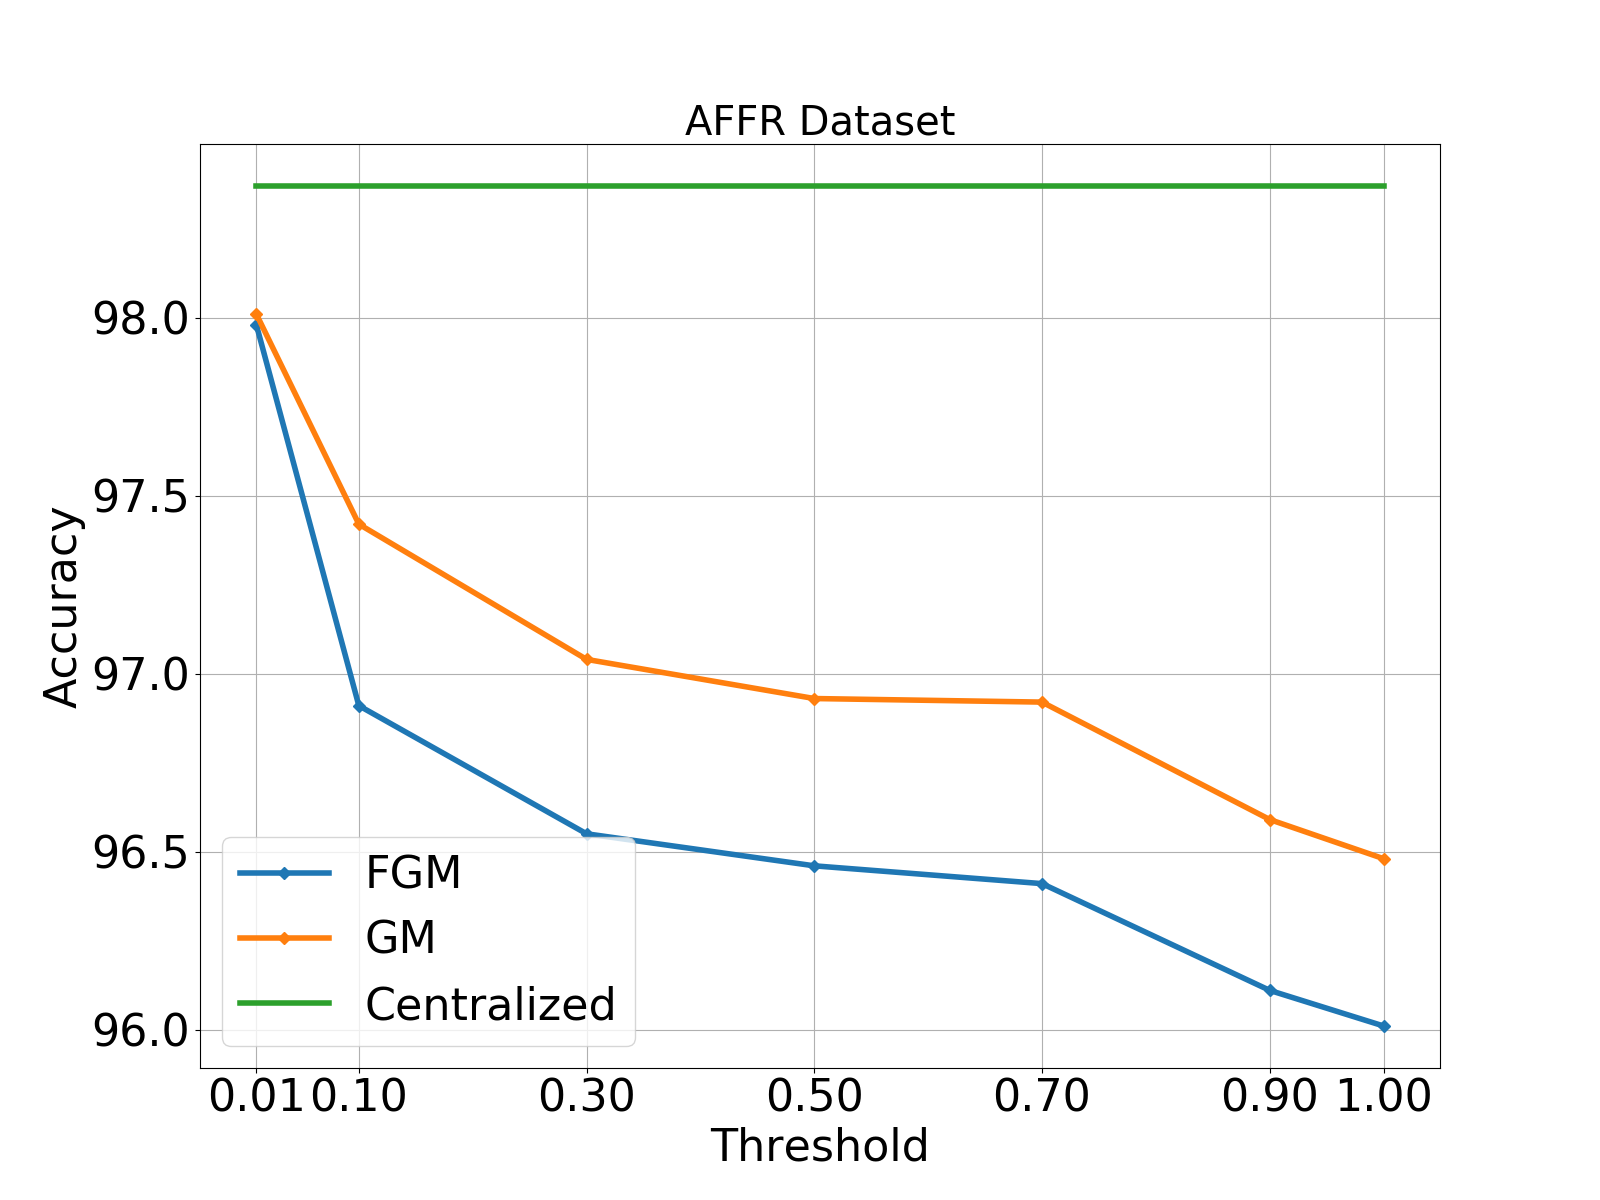
\includegraphics[width=\textwidth]{./images/results/amazon-plots/exp_Fig_1_1.png}
        \caption{}
    \end{subfigure}
    \begin{subfigure}[b]{0.45\textwidth}
        \centering
        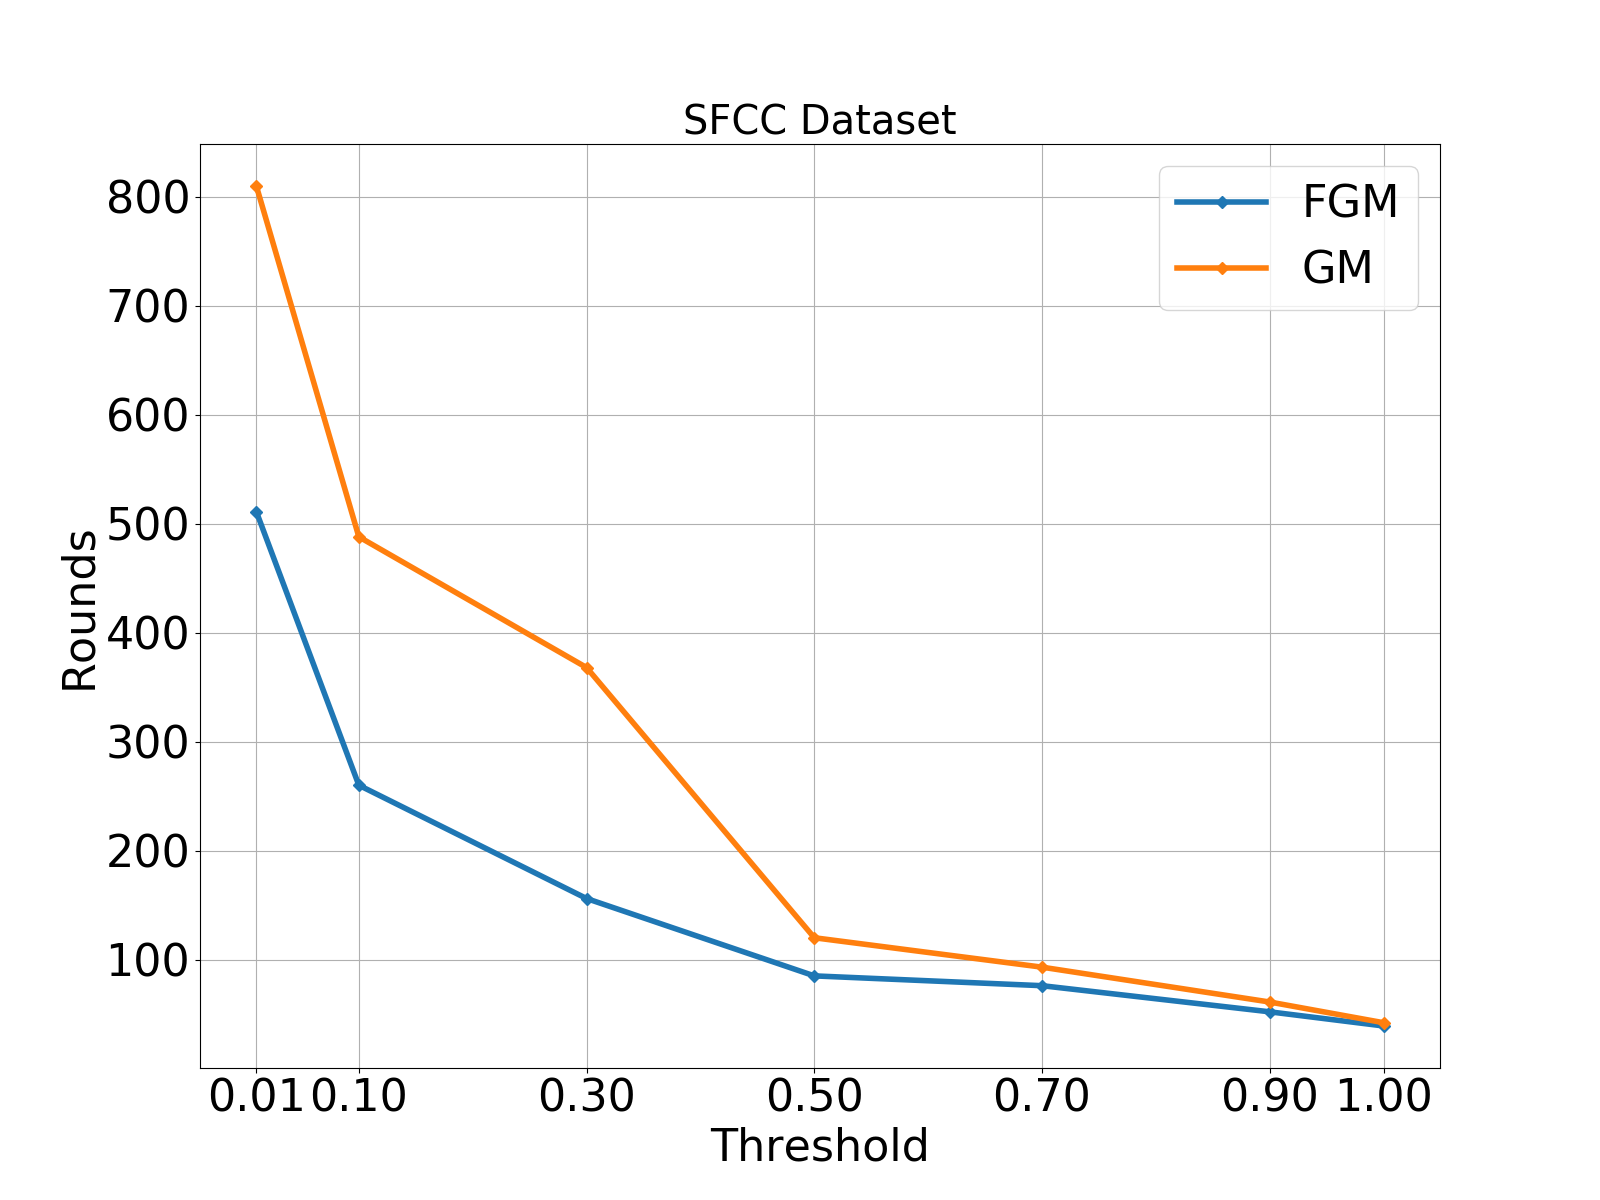
\includegraphics[width=\textwidth]{./images/results/sfc-plots/exp_Fig_1_2.png}
        \caption{}
    \end{subfigure}
    \hfill
    \begin{subfigure}[b]{0.45\textwidth}
        \centering
        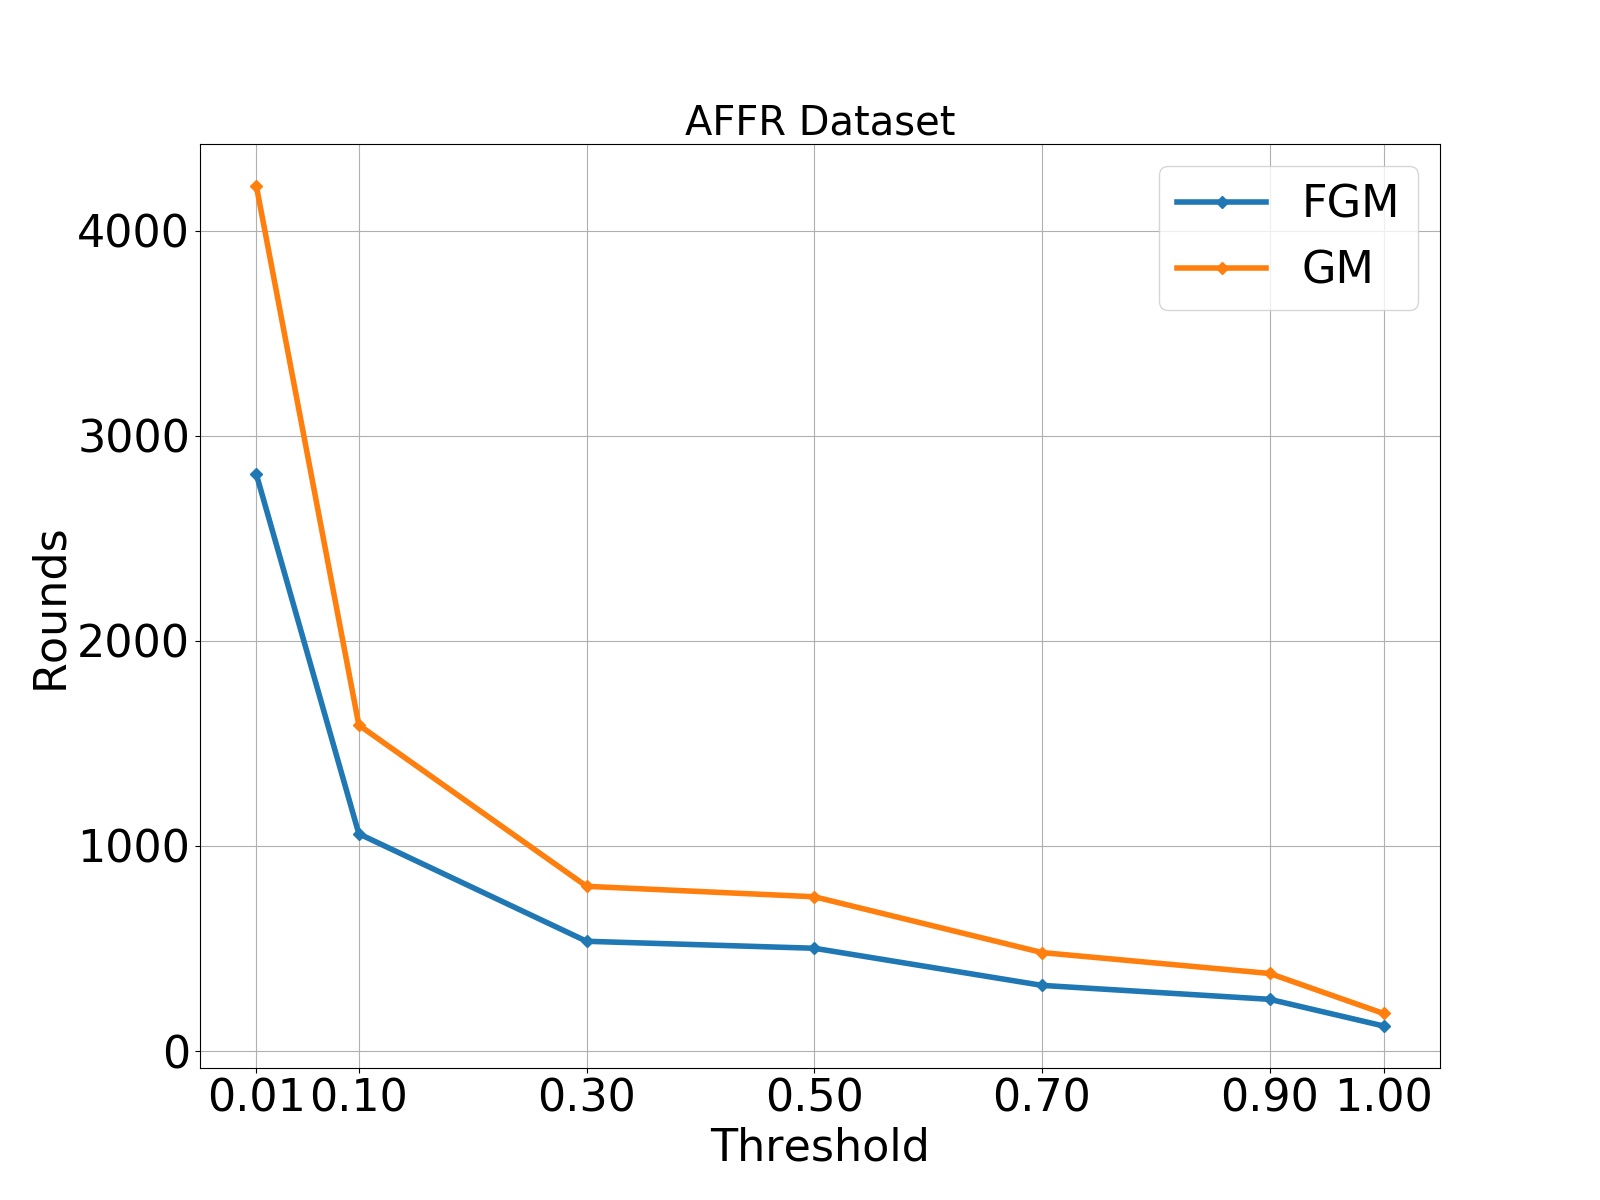
\includegraphics[width=\textwidth]{./images/results/amazon-plots/exp_Fig_1_2.png}
        \caption{}
    \end{subfigure}
    \begin{subfigure}[b]{0.45\textwidth}
        \centering
        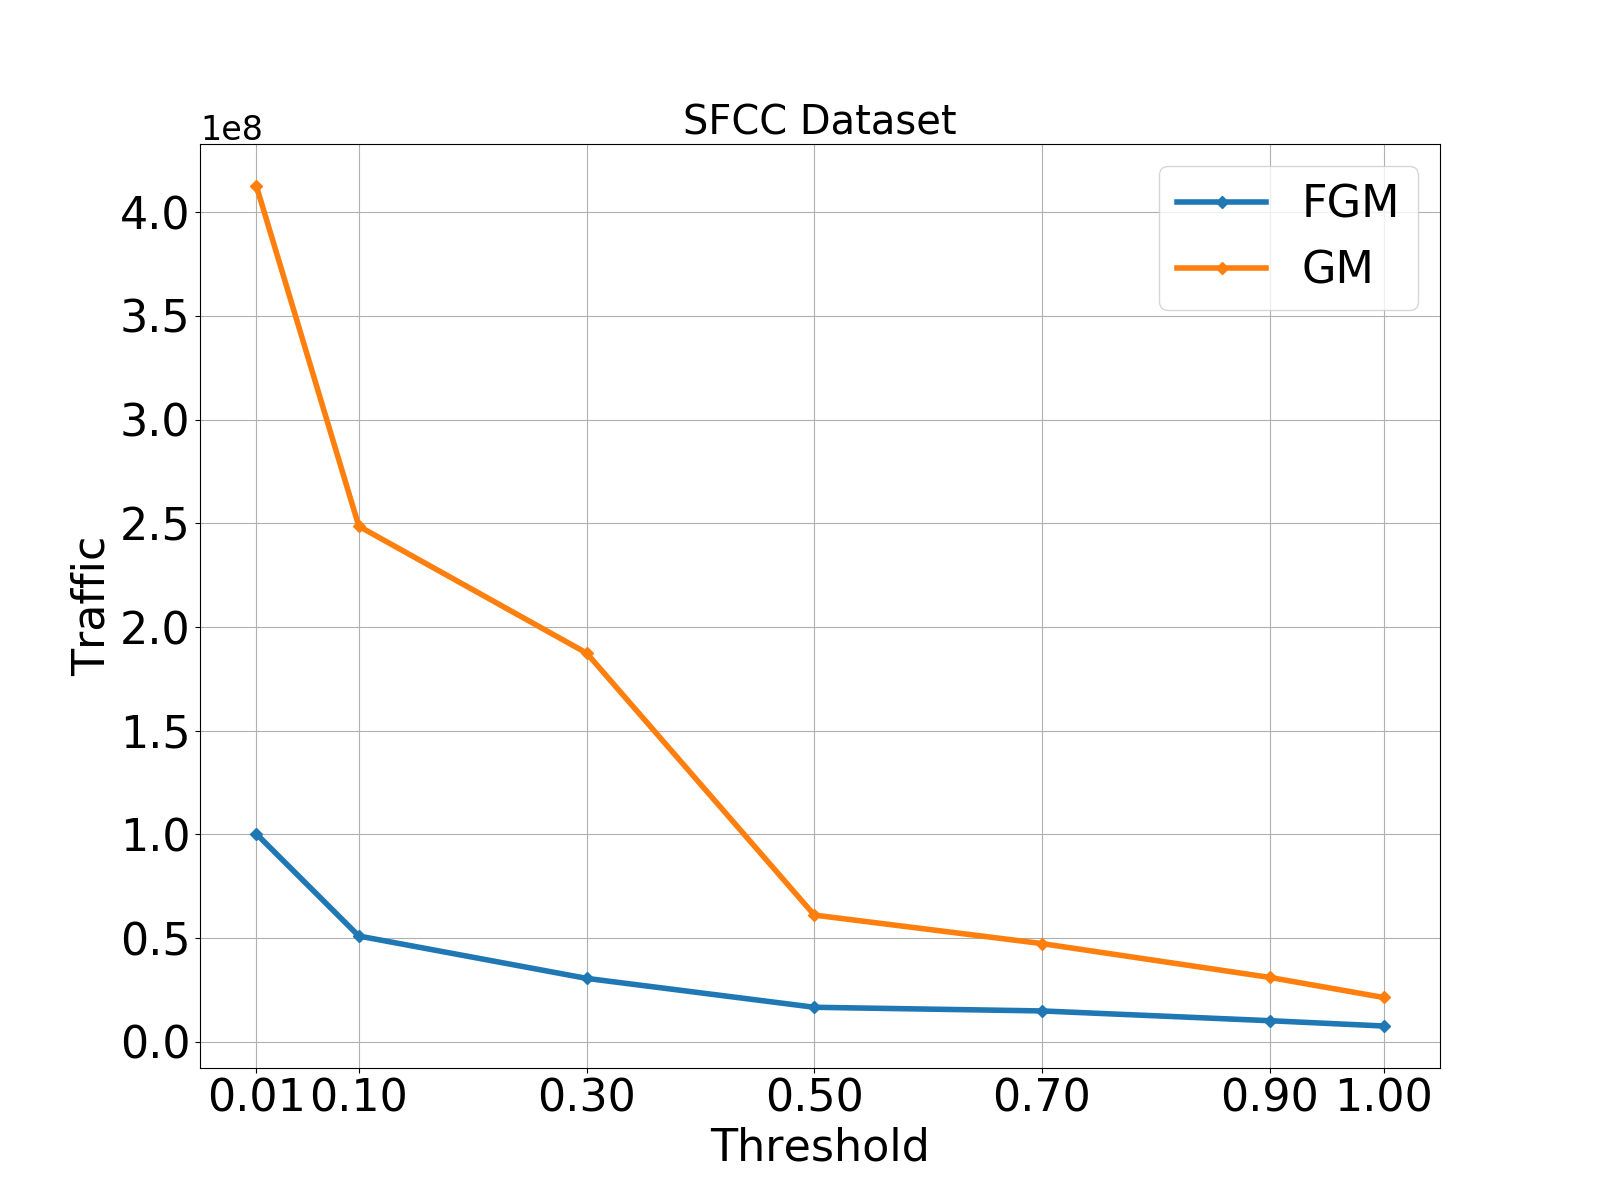
\includegraphics[width=\textwidth]{./images/results/sfc-plots/exp_Fig_1_3.png}
        \caption{}
    \end{subfigure}
    \hfill
    \begin{subfigure}[b]{0.45\textwidth}
        \centering
        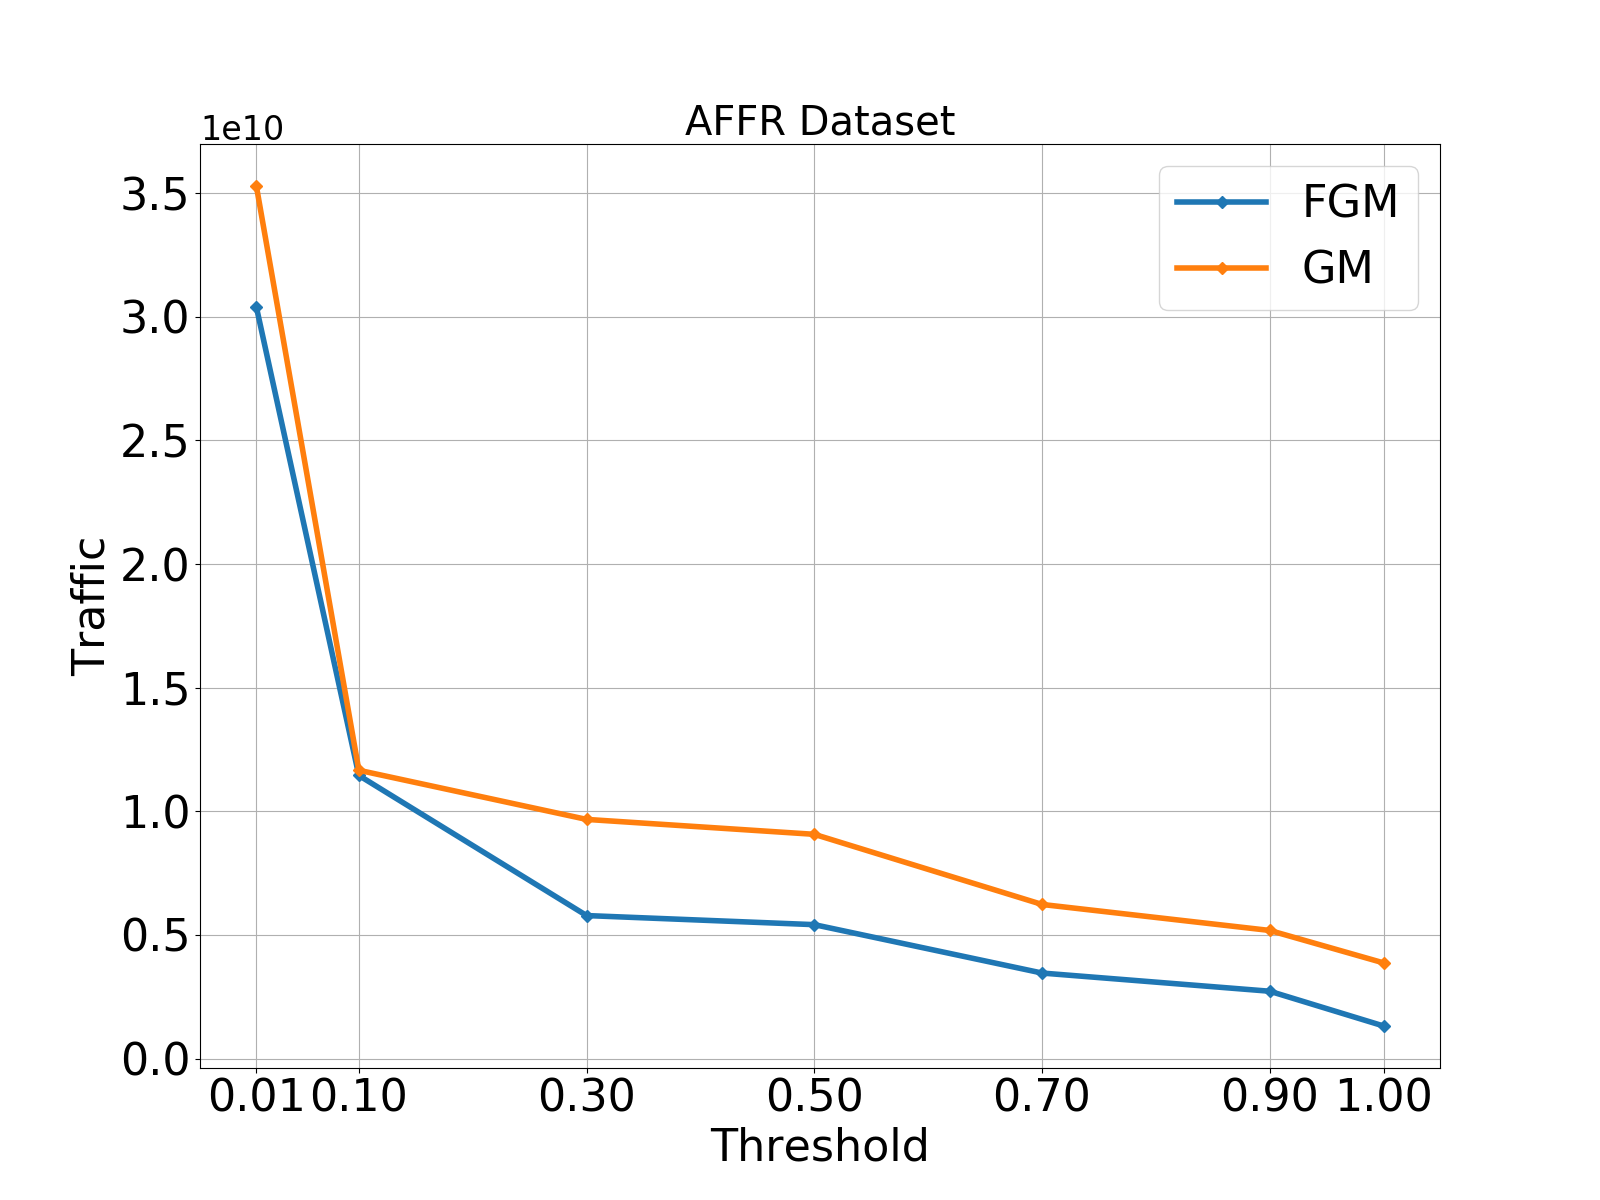
\includegraphics[width=\textwidth]{./images/results/amazon-plots/exp_Fig_1_3.png}
        \caption{}
    \end{subfigure}
    \caption{}
    \label{fig:sfcc-affr_1}
\end{figure}

\newpage

Before a worker calculates its new drift vector, it fits to the local model a batch of samples.
In this subgroup, the variable that changes is the batch size.
It is very interesting that the accuracy in SFCC is precisely the same (Fig.~\ref{fig:sfcc-affr_2_1} A).
In AFFR (Fig.~\ref{fig:sfcc-affr_2_1} B), the FGM is better than GM, but the difference is just $0.5\%$ which is a negligible amount.

\begin{figure}[H]
    \centering
    \begin{subfigure}[b]{0.45\textwidth}
        \centering
        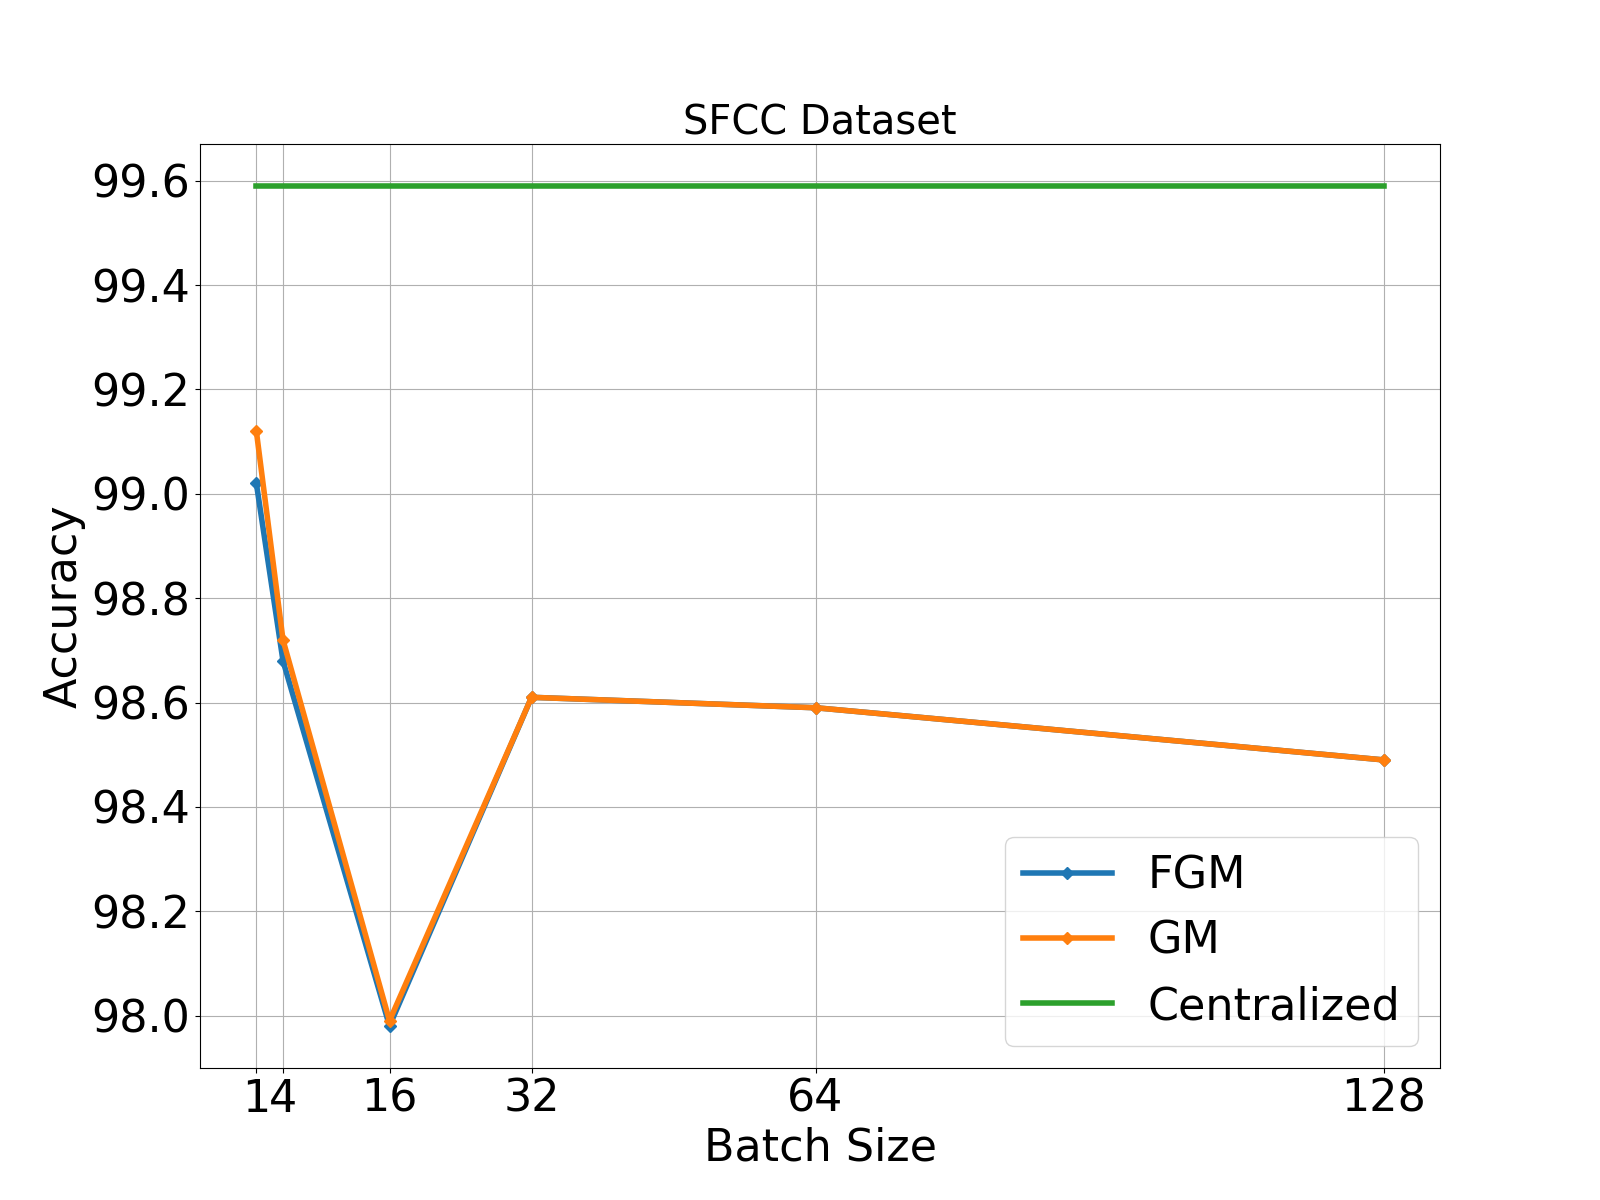
\includegraphics[width=\textwidth]{./images/results/sfc-plots/exp_Fig_2_1.png}
        \caption{}
    \end{subfigure}
    \hfill
    \begin{subfigure}[b]{0.45\textwidth}
        \centering
        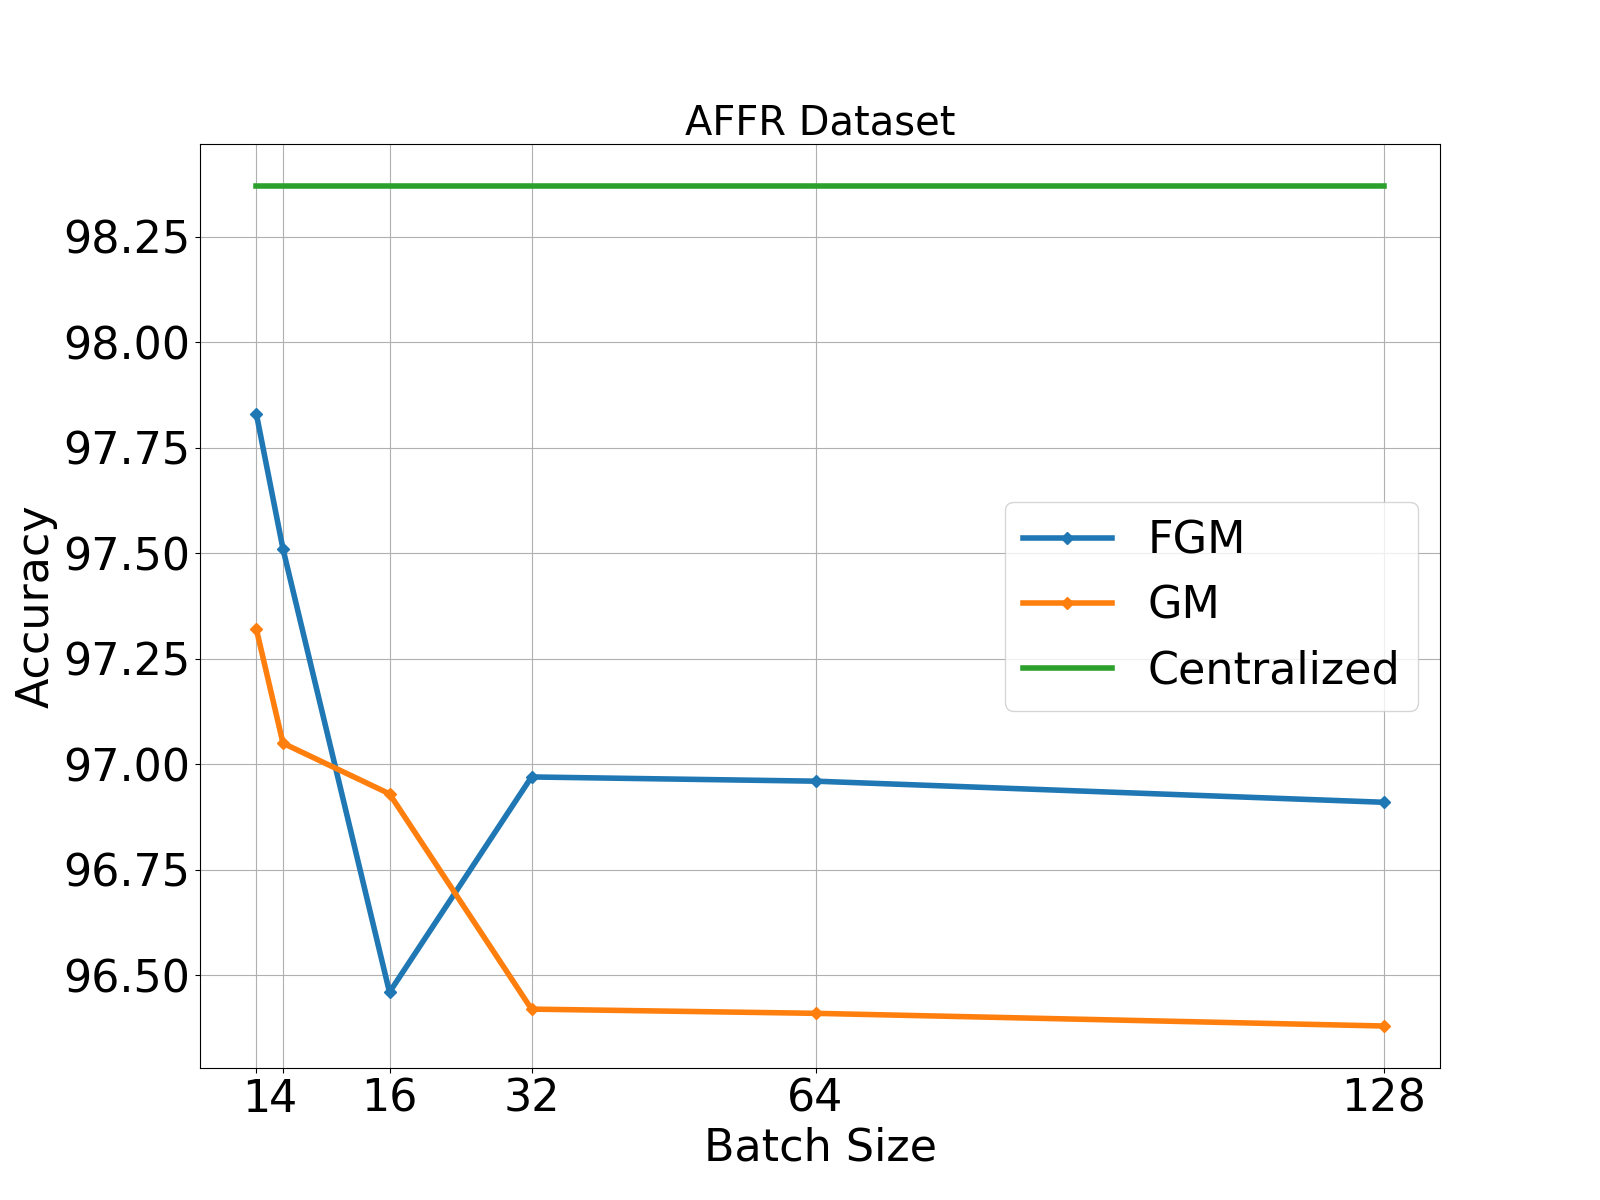
\includegraphics[width=\textwidth]{./images/results/amazon-plots/exp_Fig_2_1.png}
        \caption{}
    \end{subfigure}
    \caption{}
    \label{fig:sfcc-affr_2_1}
\end{figure}

As in the graph above with the rounds when the threshold was changing, it is acceptable that the rounds decrease while the batch size increases (Fig.~\ref{fig:sfcc-affr_2_2_2_3} A,B).
Regarding the network traffic while batch size increasing (Fig.~\ref{fig:sfcc-affr_2_2_2_3} C,D), note that the traffic is decreasing with a smaller rate due to subrounds of FGM\@.
FGM is $3.5$ times more efficient than GM in SFCC\@.
In AFFR, the percentage change is $100\%$.

\begin{figure}[H]
    \centering
    \begin{subfigure}[b]{0.45\textwidth}
        \centering
        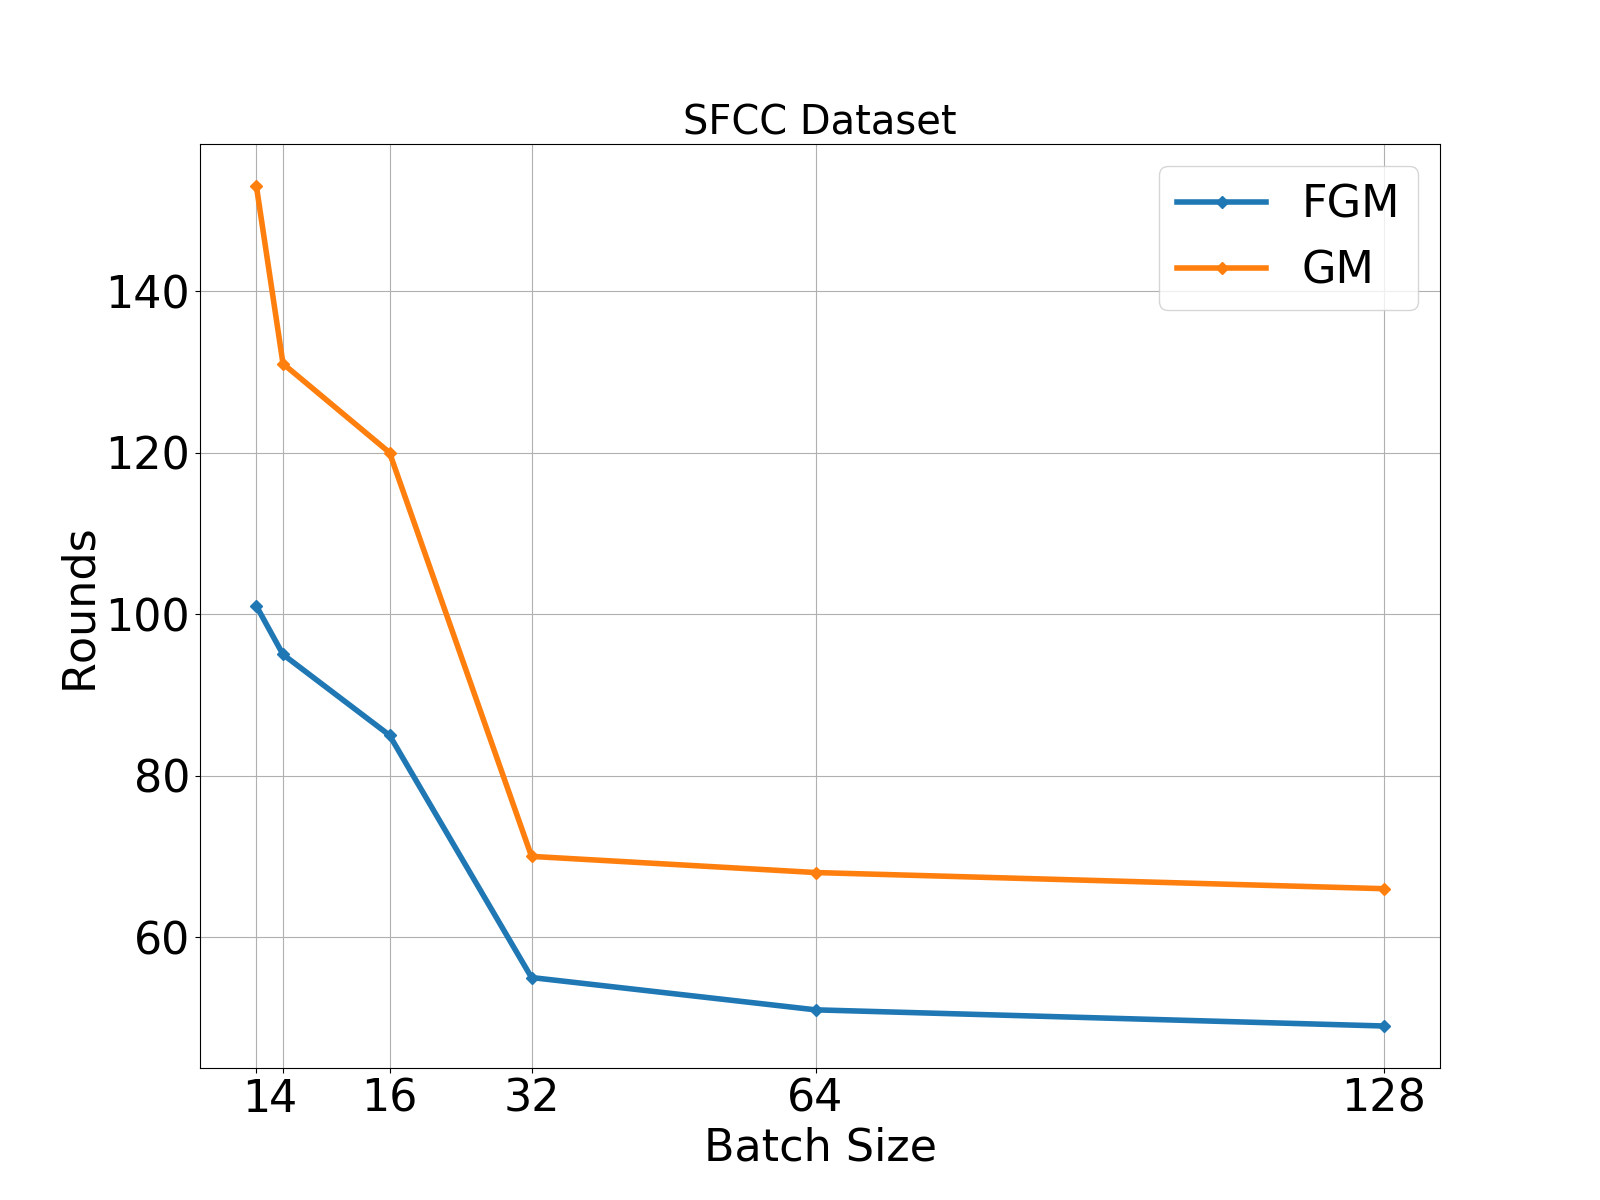
\includegraphics[width=\textwidth]{./images/results/sfc-plots/exp_Fig_2_2.png}
        \caption{}
    \end{subfigure}
    \hfill
    \begin{subfigure}[b]{0.45\textwidth}
        \centering
        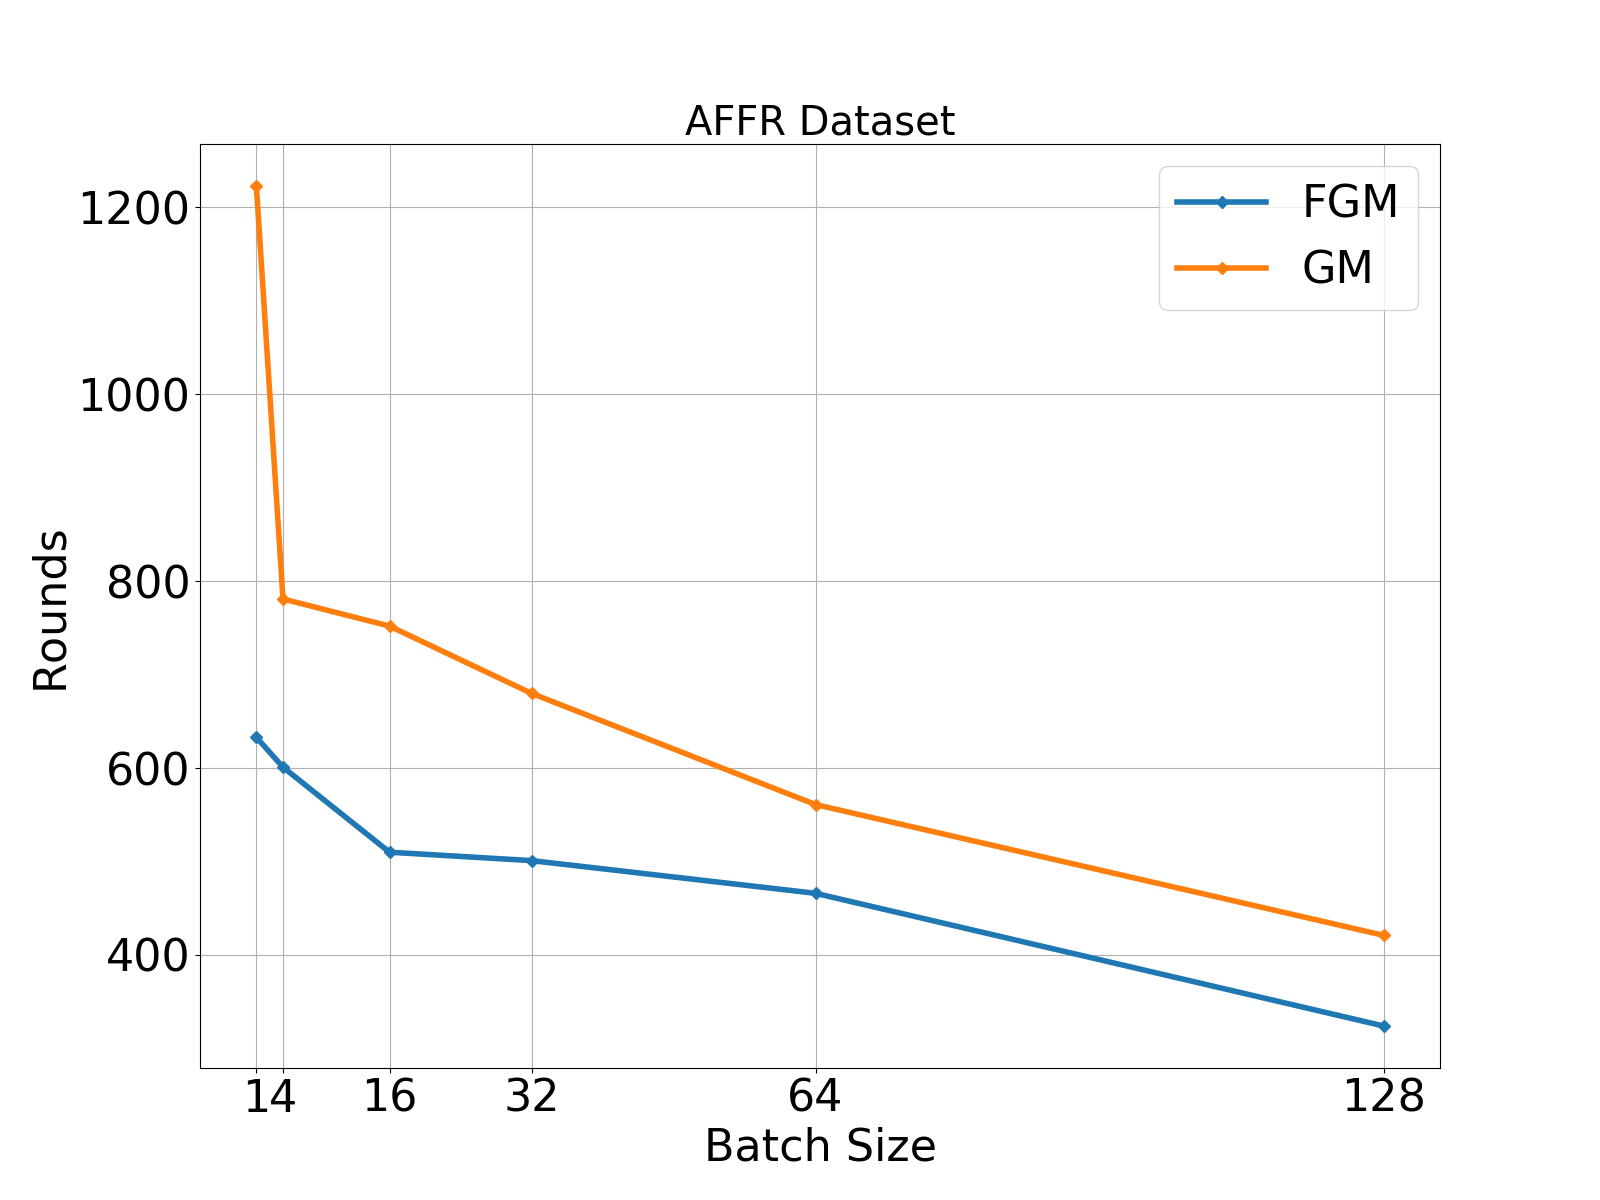
\includegraphics[width=\textwidth]{./images/results/amazon-plots/exp_Fig_2_2.png}
        \caption{}
    \end{subfigure}
    \begin{subfigure}[b]{0.45\textwidth}
        \centering
        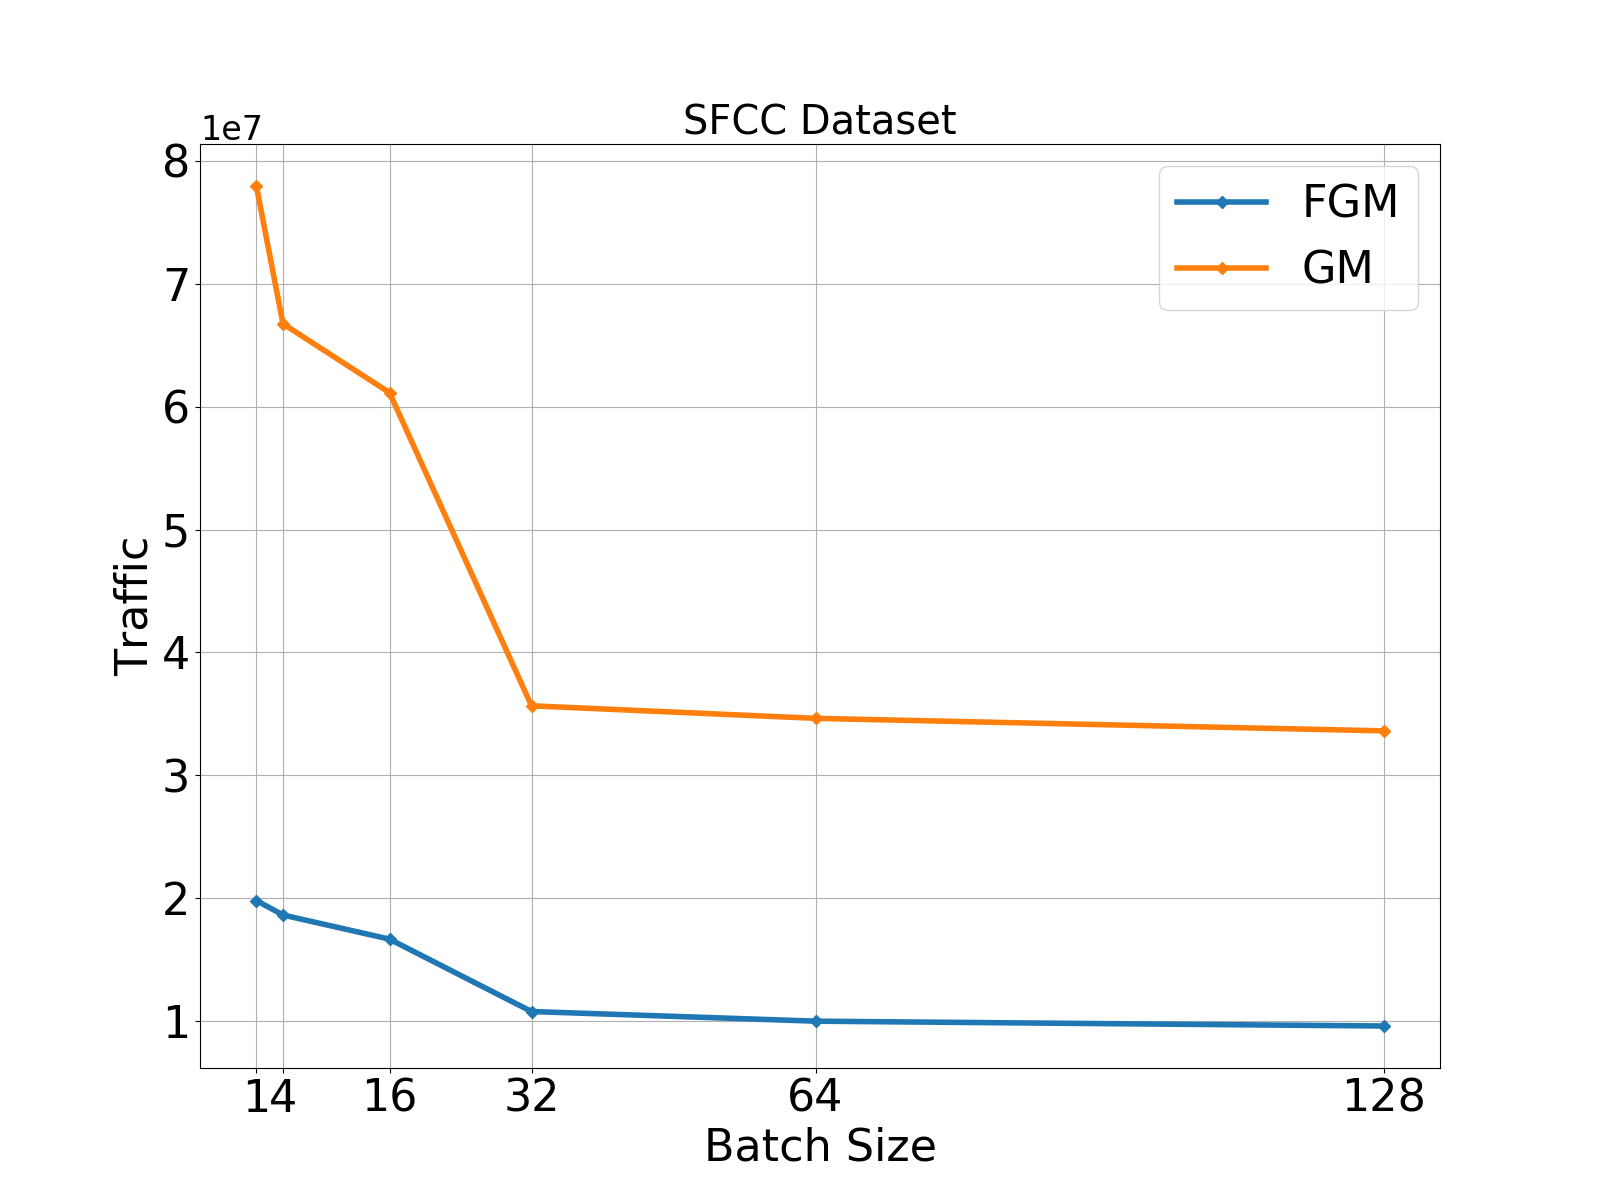
\includegraphics[width=\textwidth]{./images/results/sfc-plots/exp_Fig_2_3.png}
        \caption{}
    \end{subfigure}
    \hfill
    \begin{subfigure}[b]{0.45\textwidth}
        \centering
        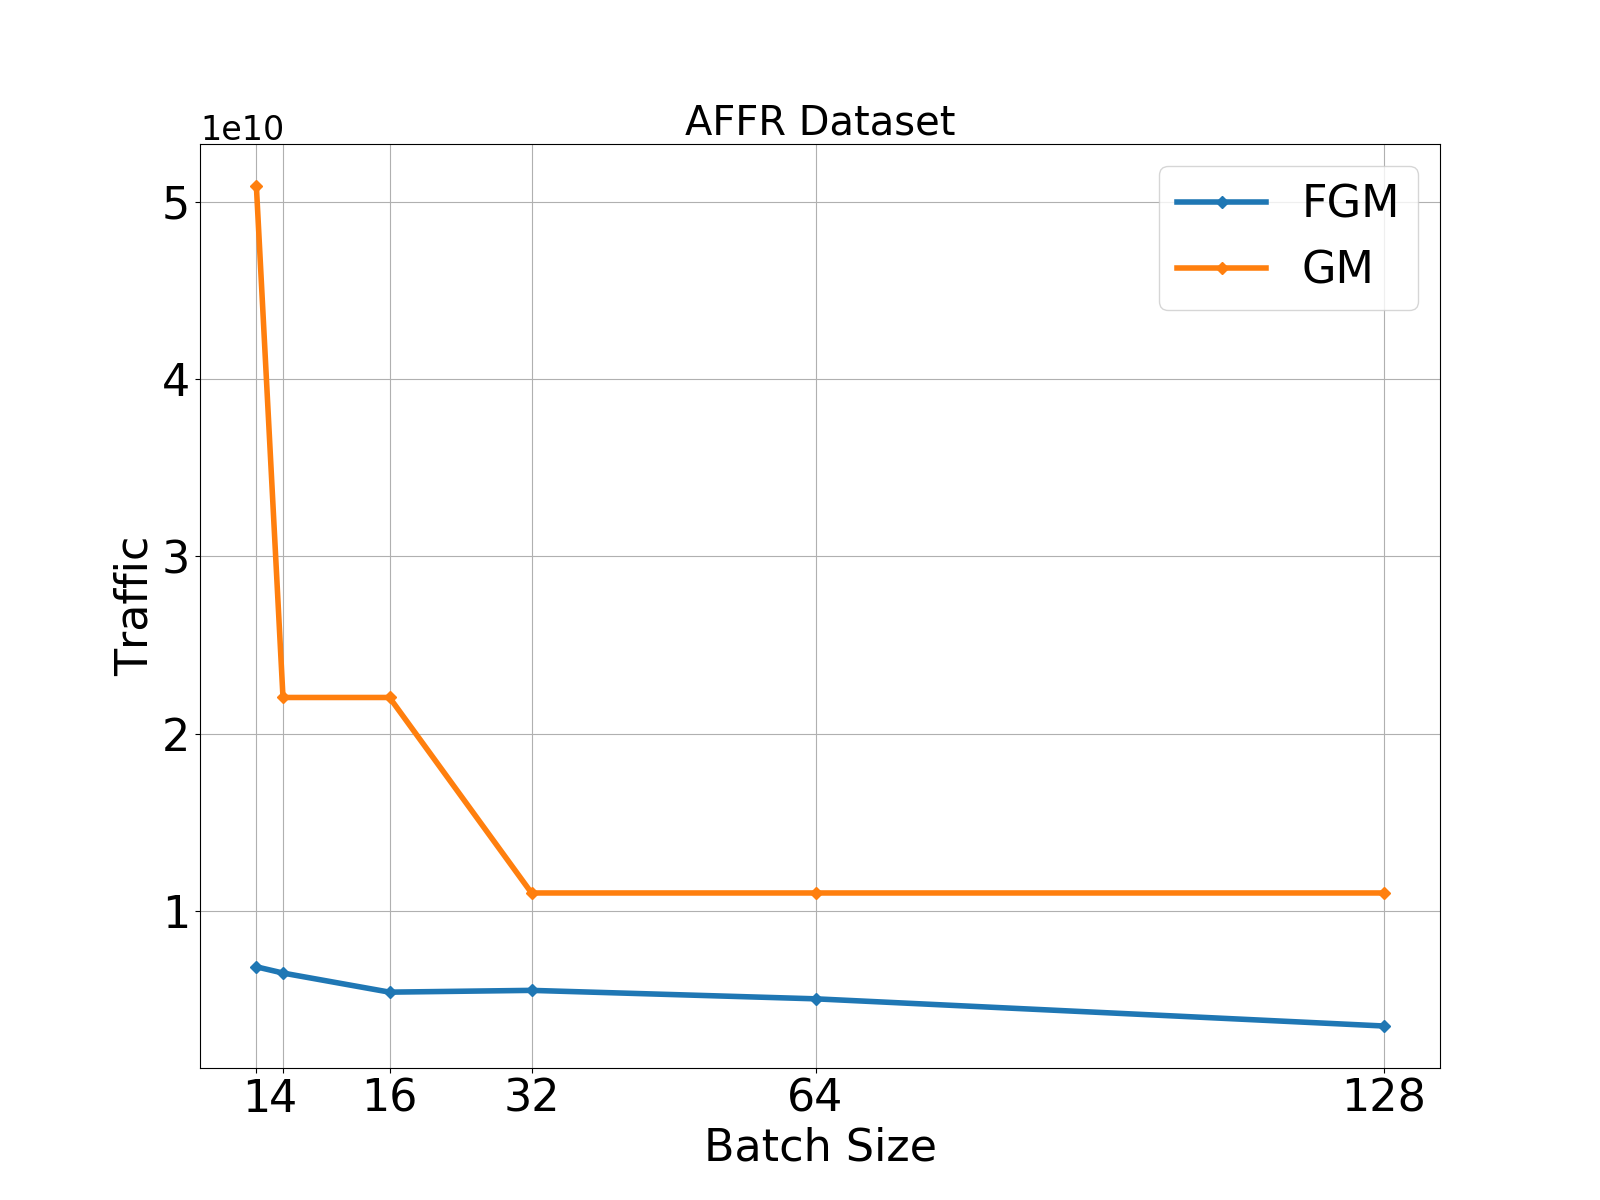
\includegraphics[width=\textwidth]{./images/results/amazon-plots/exp_Fig_2_3.png}
        \caption{}
    \end{subfigure}
    \caption{}
    \label{fig:sfcc-affr_2_2_2_3}
\end{figure}

In SFCC and especially in the case of $8$ workers, we see probably an outlier (Fig.~\ref{fig:sfcc-affr_3_1} A,B).
After that, the accuracy decreases over the increase of scalability, but not too much to make a problem.
In AFFR, there is no outlier and the accuracy follows the expected direction.
Here FGM is more precise than GM by $0.5\%$.

\begin{figure}[H]
    \centering
    \begin{subfigure}[b]{0.45\textwidth}
        \centering
        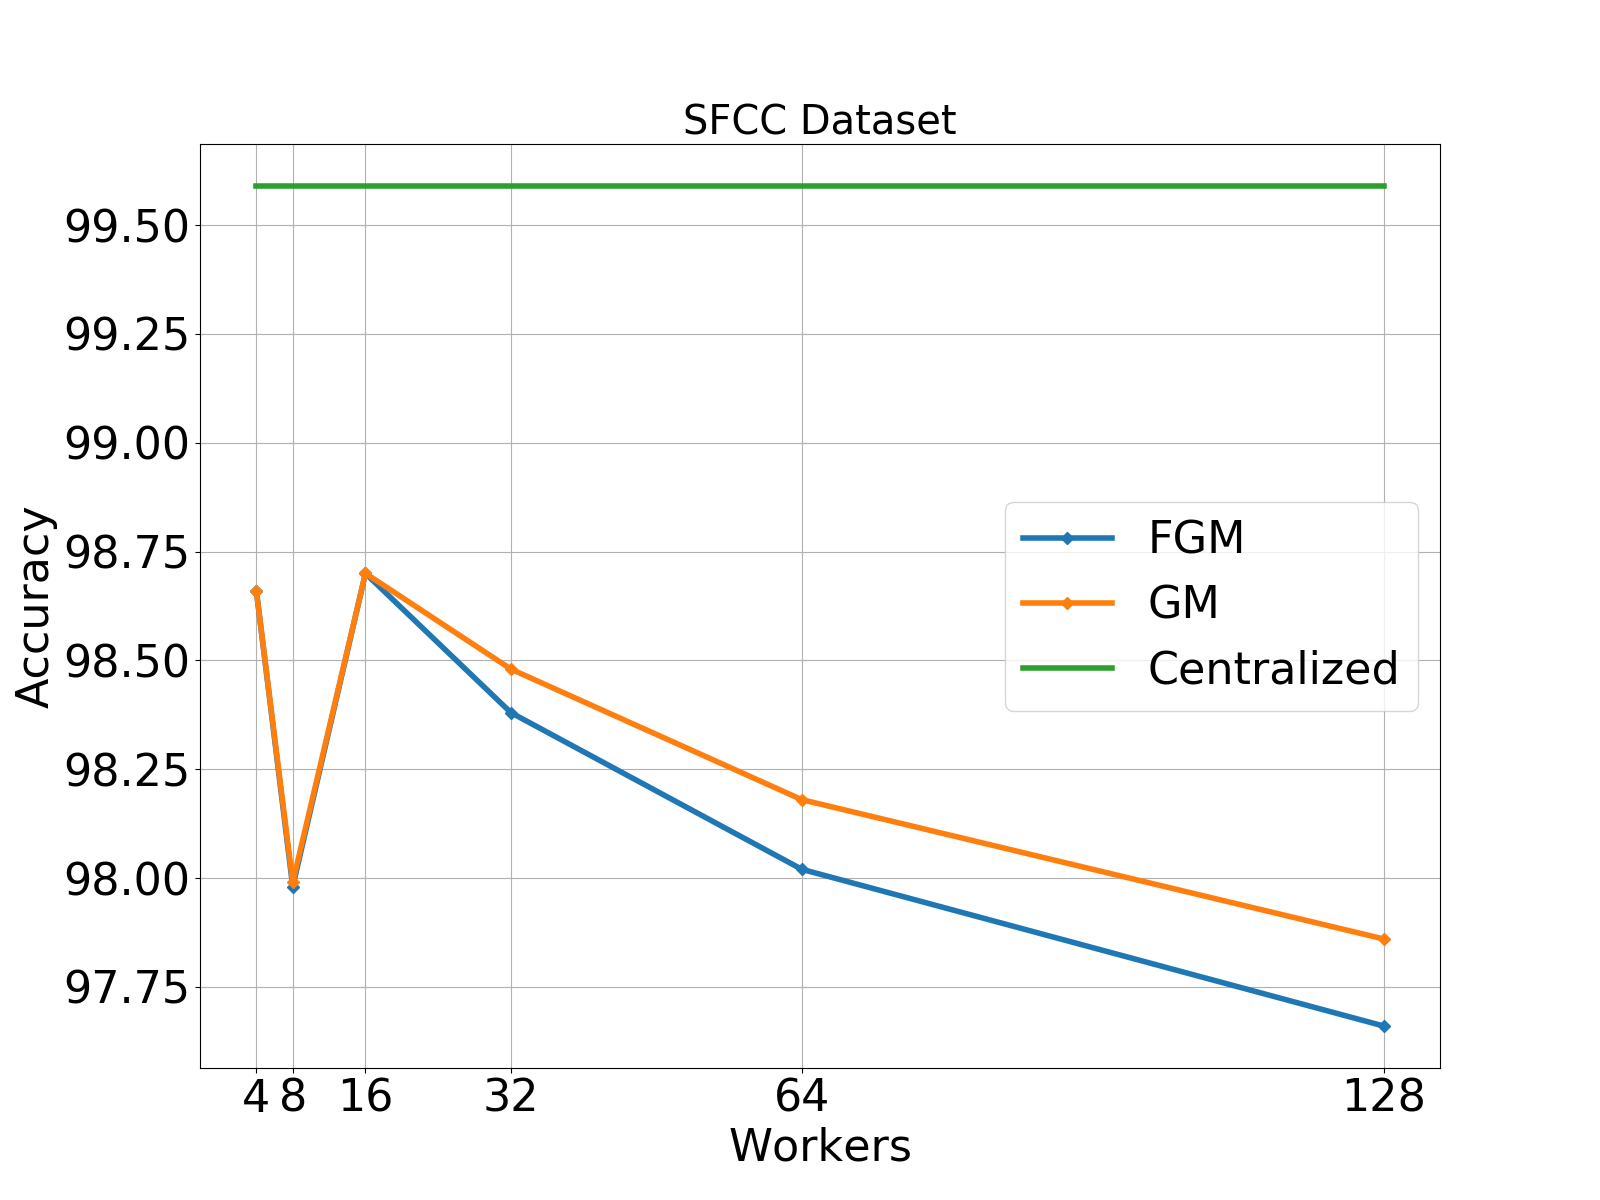
\includegraphics[width=\textwidth]{./images/results/sfc-plots/exp_Fig_3_1.png}
        \caption{}
    \end{subfigure}
    \hfill
    \begin{subfigure}[b]{0.45\textwidth}
        \centering
        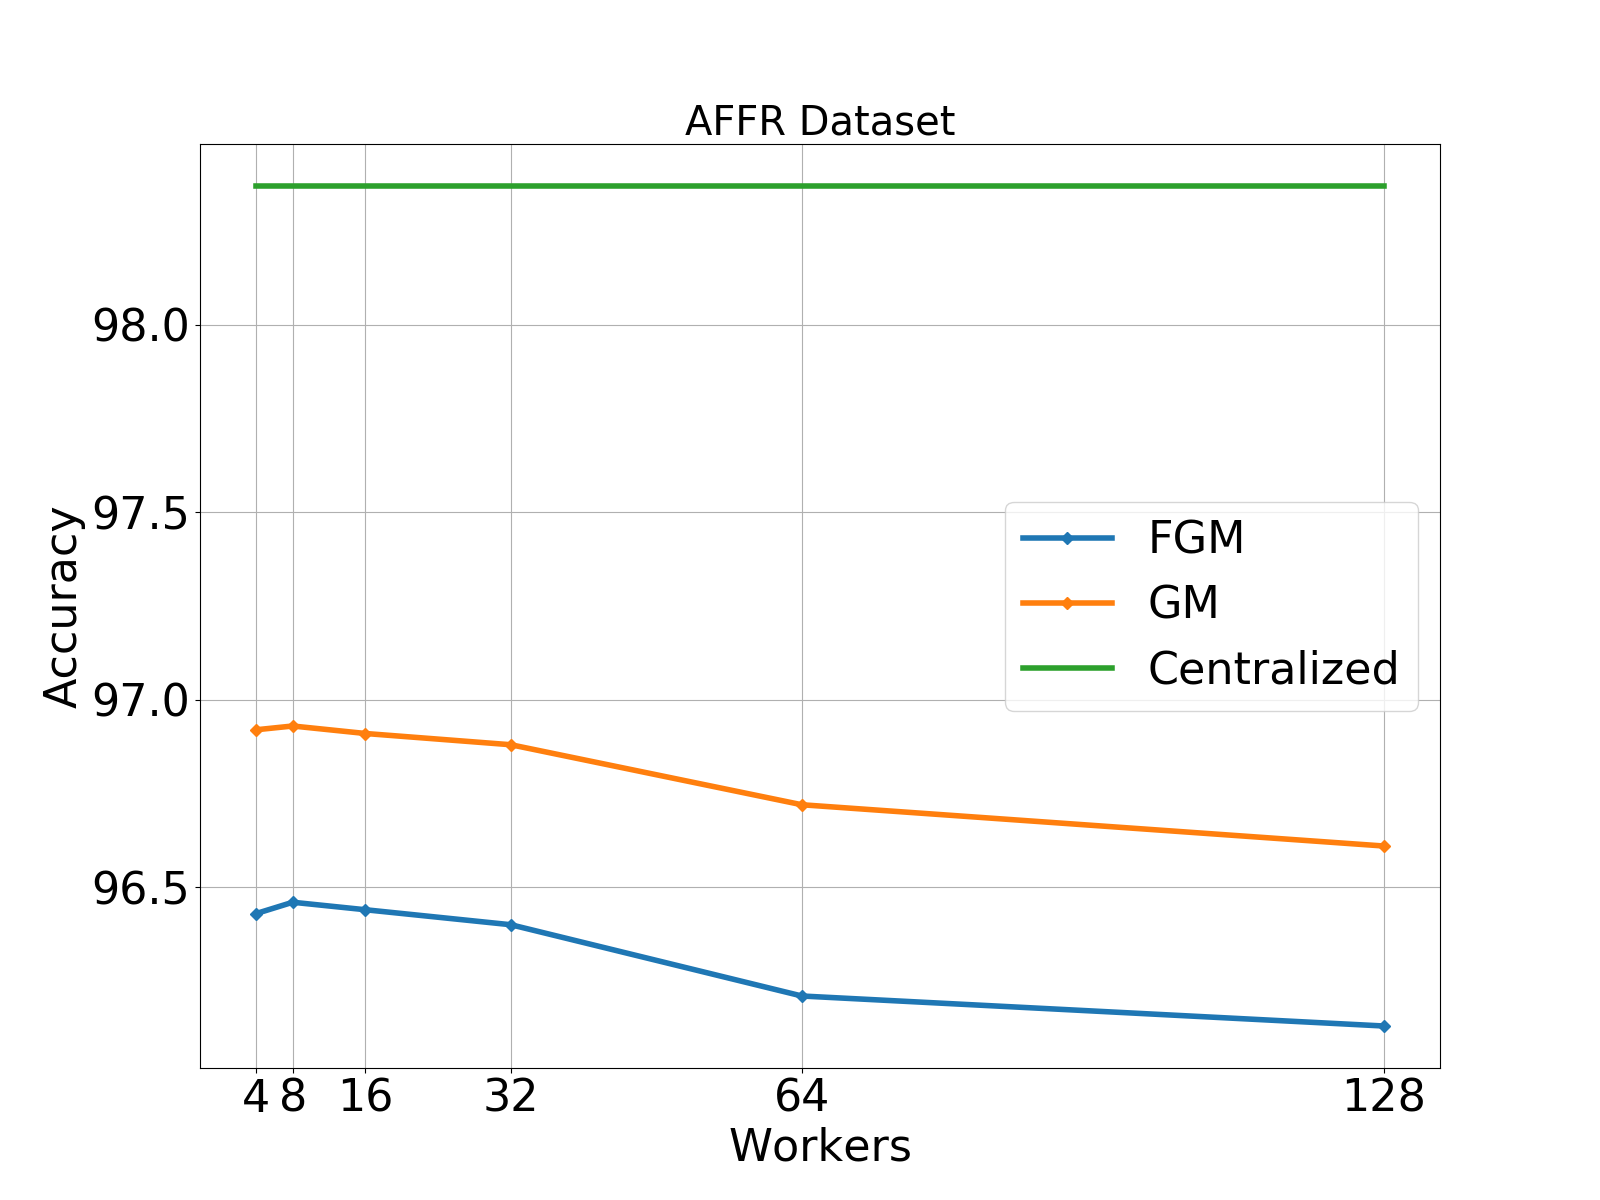
\includegraphics[width=\textwidth]{./images/results/amazon-plots/exp_Fig_3_1.png}
        \caption{}
    \end{subfigure}
    \caption{}\label{fig:sfcc-affr_3_1}
\end{figure}

In Figure~\ref{fig:sfcc-affr_3_2} A,B, it seems that both models follow the same direction.
The rounds decrease over the increase of workers.
Again the class model achieves fewer rounds than NLP\@.

\begin{figure}[H]
    \centering
    \begin{subfigure}[b]{0.45\textwidth}
        \centering
        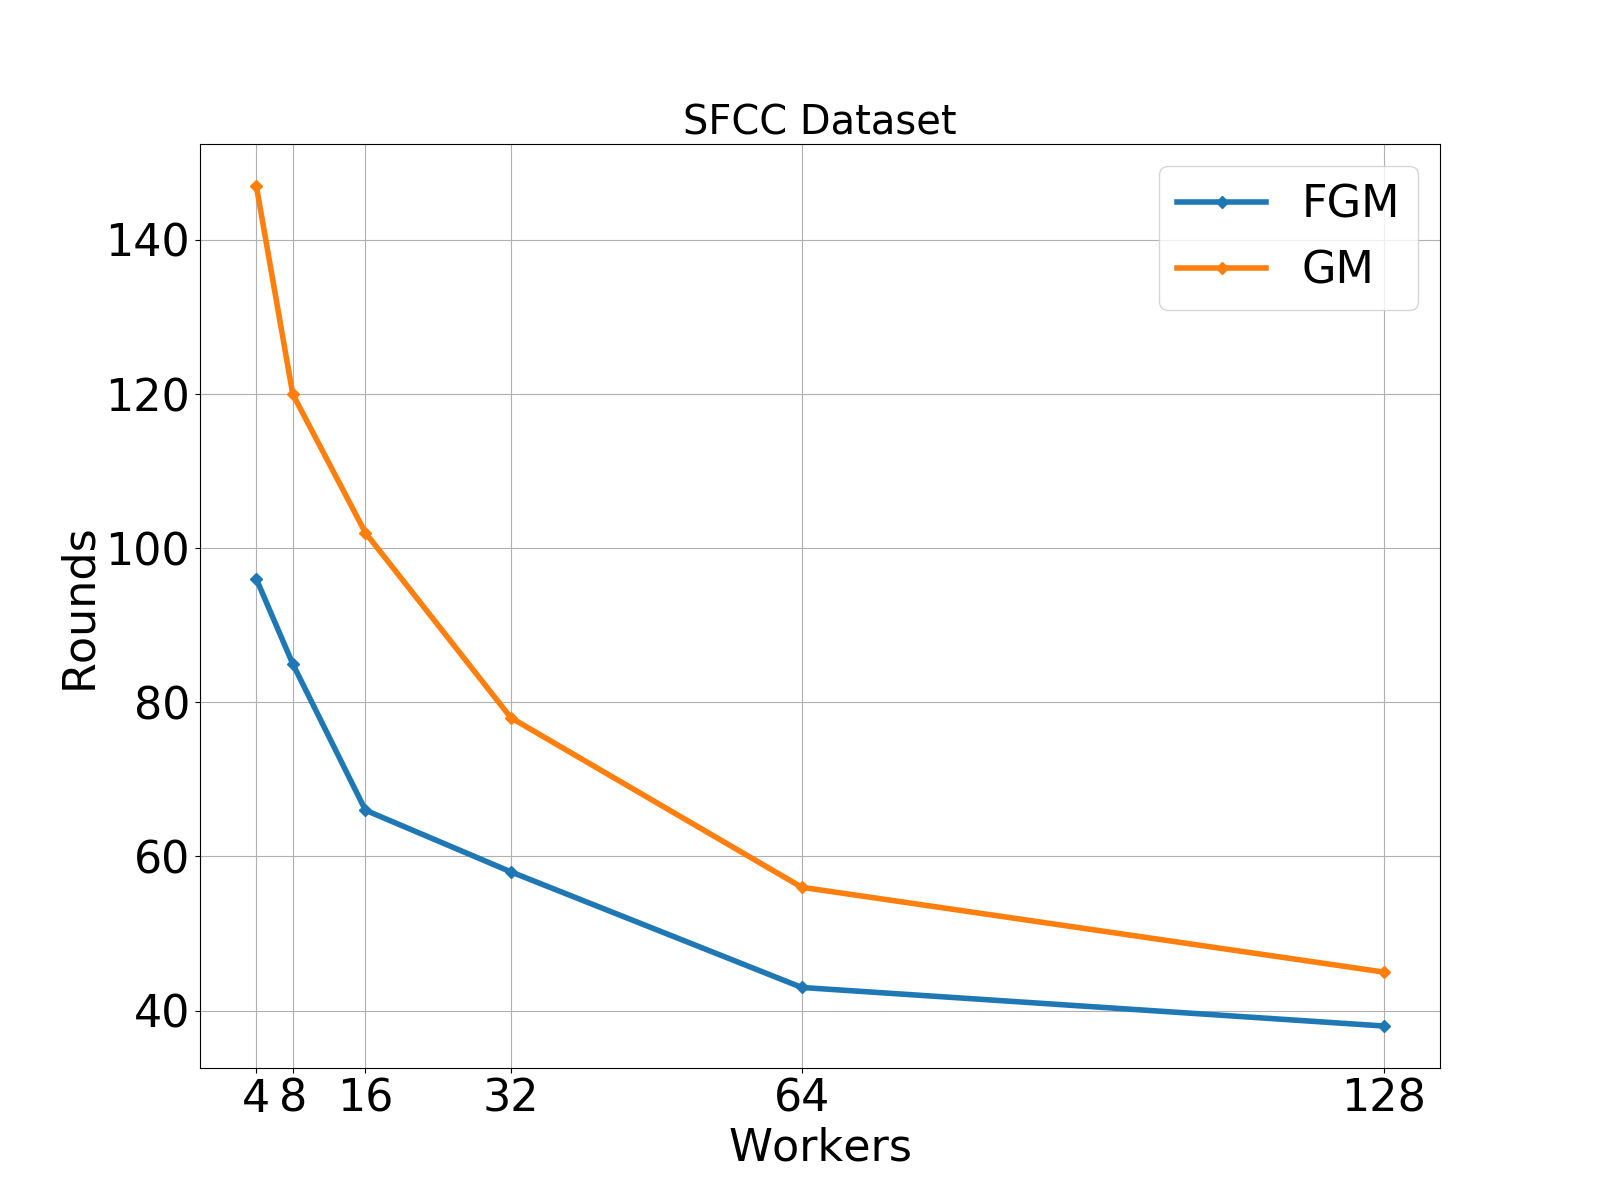
\includegraphics[width=\textwidth]{./images/results/sfc-plots/exp_Fig_3_2.png}
        \caption{}
    \end{subfigure}
    \hfill
    \begin{subfigure}[b]{0.45\textwidth}
        \centering
        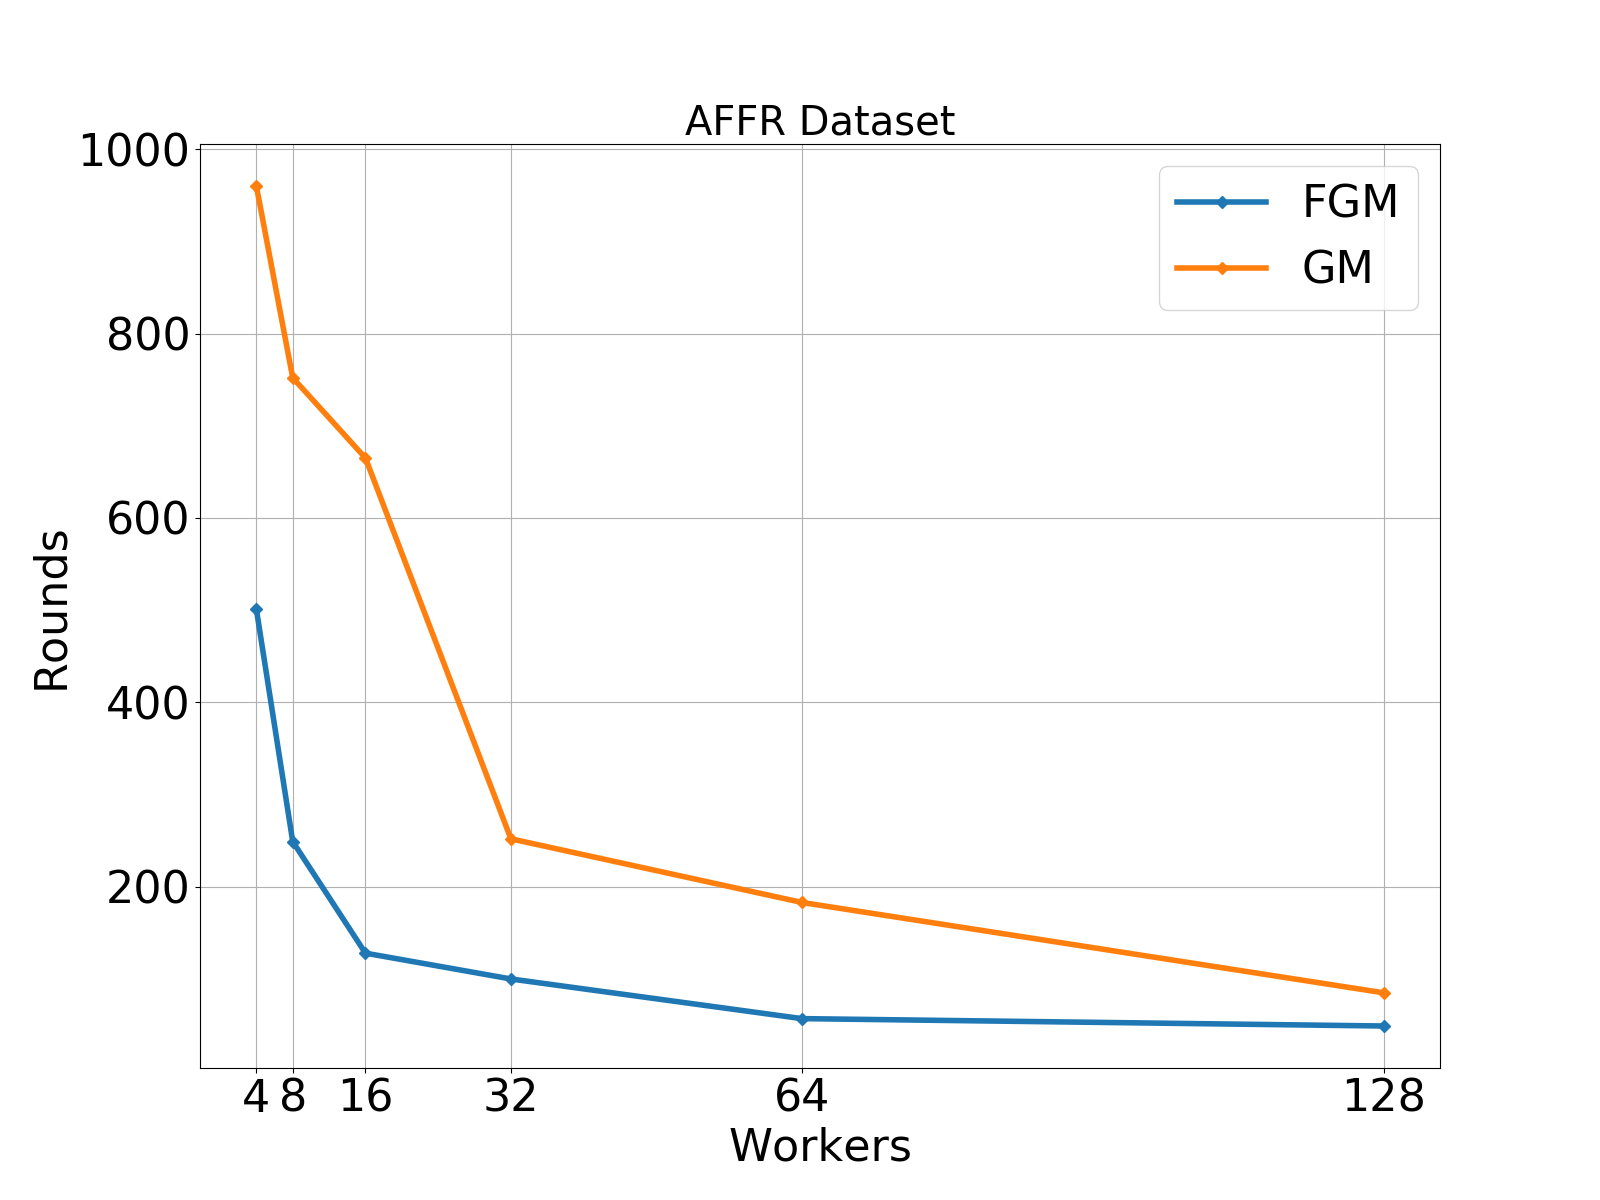
\includegraphics[width=\textwidth]{./images/results/amazon-plots/exp_Fig_3_2.png}
        \caption{}
    \end{subfigure}
    \caption{}
    \label{fig:sfcc-affr_3_2}
\end{figure}

\newpage

These plots (Fig.~\ref{fig:sfcc-affr_3_3} A,B) are typical GM-FGM plots on scalability analysis.
FGM keeps the same levels of traffic while the workers are increasing.
On the other hand, GM uses more network resources while the network getting bigger.
FGM is up to $7$ times more efficient than GM in SFCC and up to $15$ in AFFR\@.
NLP problems fit better to this architecture.
Additionally, these plots are the most important of this work since the gap of the network cost between the two methods becomes enormous, while the accuracy remains at the same high levels in both algorithms.
The number of rounds may not be very different by absolute numbers, although this is where the superiority of FGM is located.

At this point, note that for FGM a subround costs some bytes since the only thing that needs to be transferred is the increment from the workers to the coordinator and the quantum from the coordinator to the workers.
On the other hand, a rebalance is equivalent to thousands of bytes since the workers send their entire model to the coordinator.
Therefore, it seems that as the number of workers increases, the communication in GM increases linearly while in FGM it remains relatively stable.

\begin{figure}[H]
    \centering
    \begin{subfigure}[b]{0.45\textwidth}
        \centering
        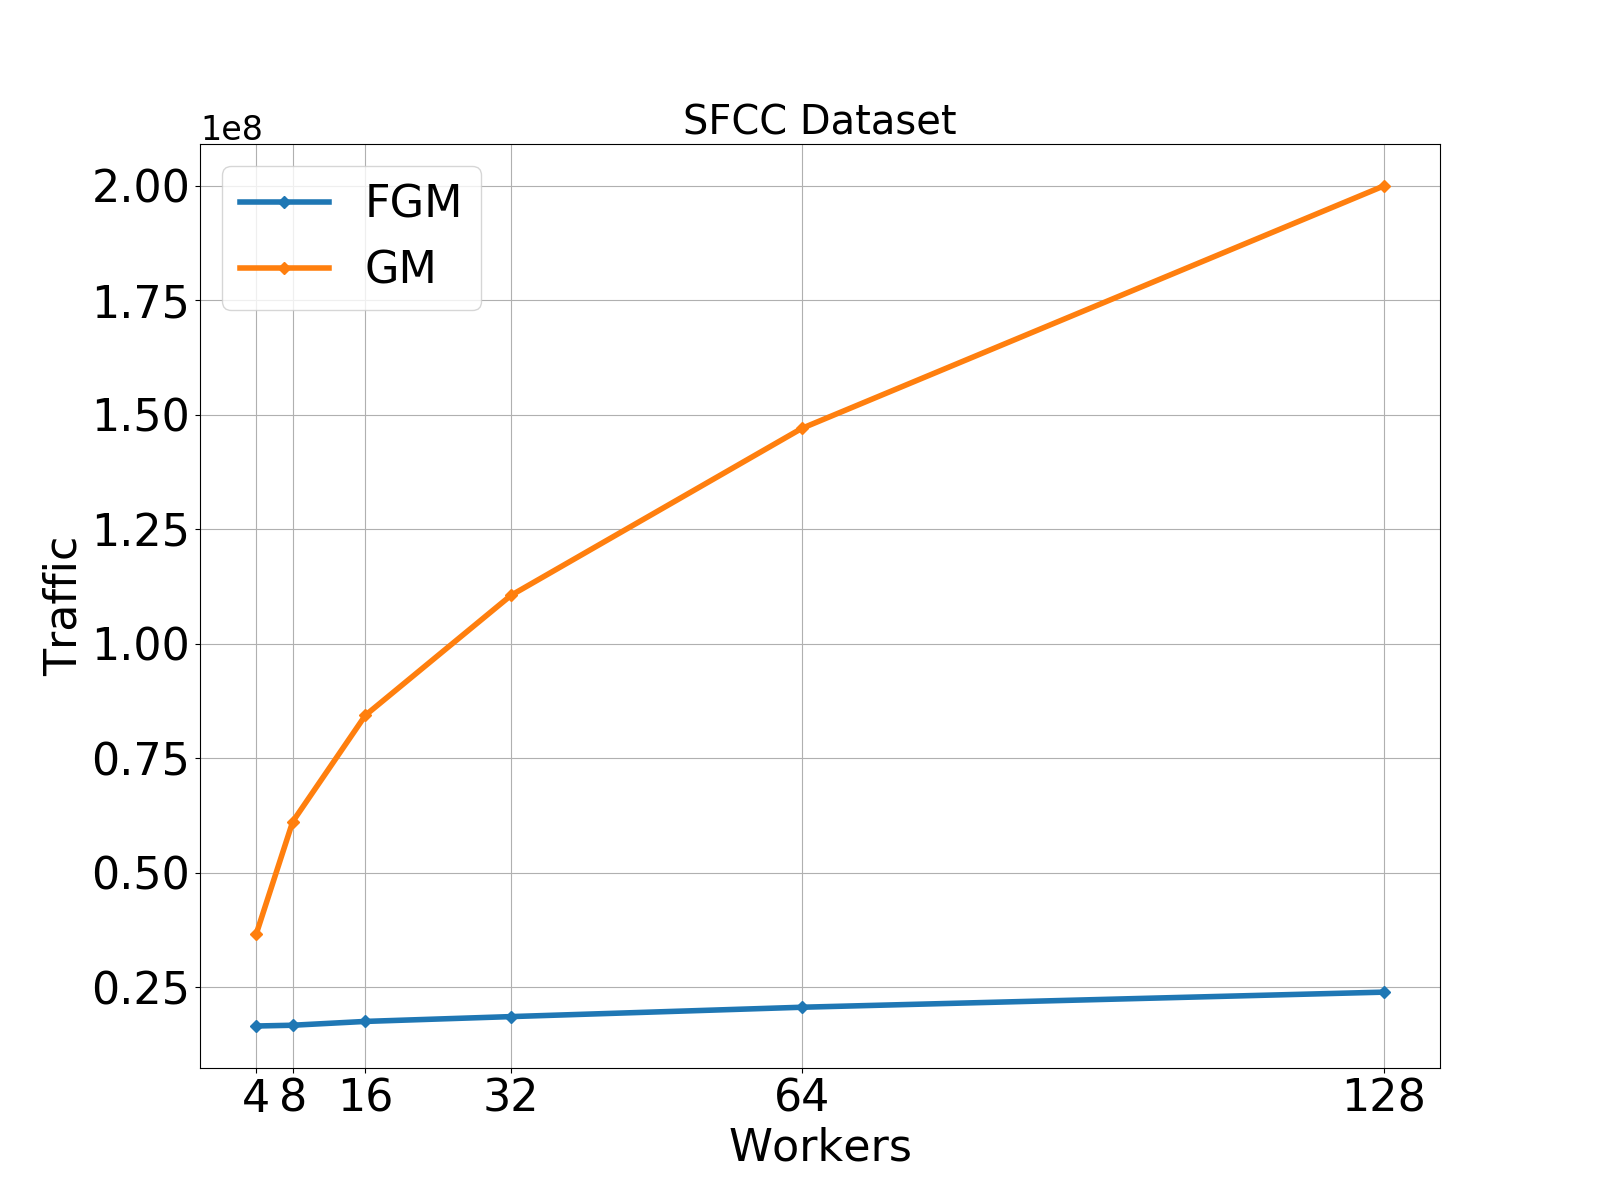
\includegraphics[width=\textwidth]{./images/results/sfc-plots/exp_Fig_3_3.png}
        \caption{}
    \end{subfigure}
    \hfill
    \begin{subfigure}[b]{0.45\textwidth}
        \centering
        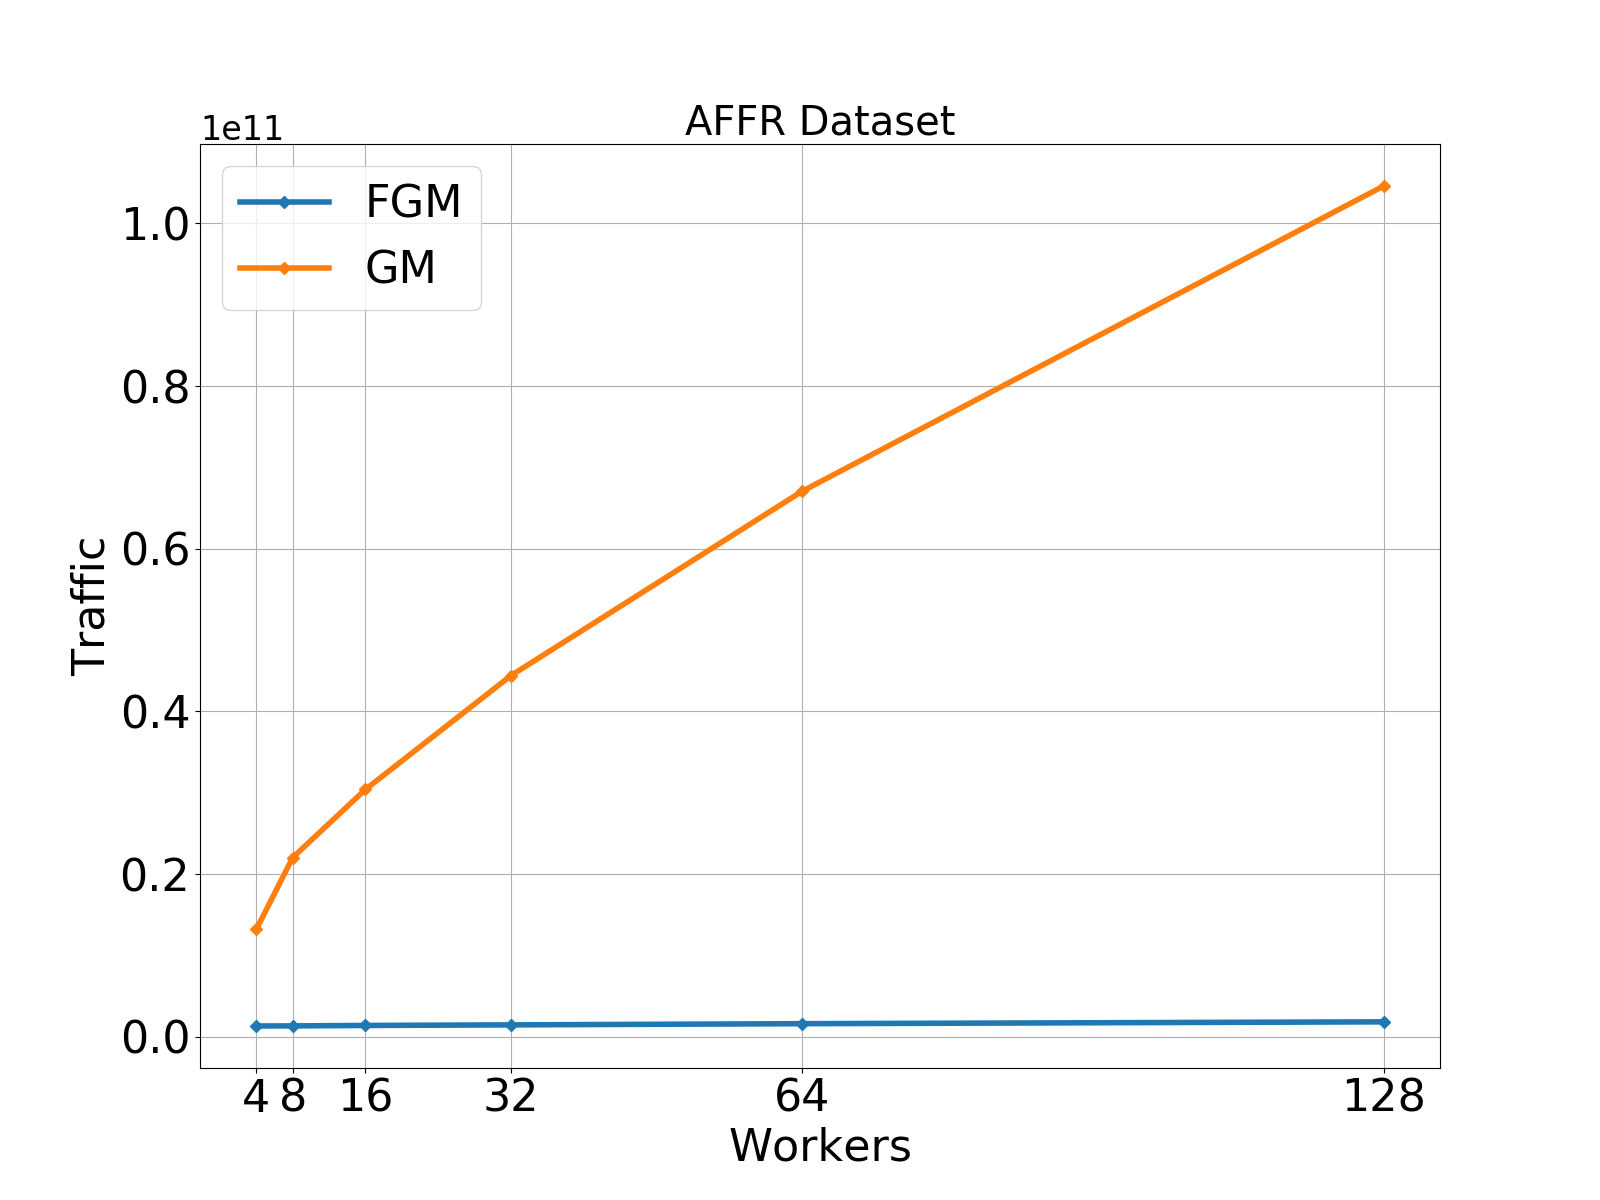
\includegraphics[width=\textwidth]{./images/results/amazon-plots/exp_Fig_3_3.png}
        \caption{}
    \end{subfigure}
    \caption{}
    \label{fig:sfcc-affr_3_3}
\end{figure}

When I collected the experiments results, I and my professor noted that it would be interesting to show the above scenario for SFCC dataset for threshold equal to $0.1$.
Seeing the below figures, the most significant plot is in the figure~\ref{fig:sfcc_3_b} C, as the others follows the same direction having an absolute difference.
So, we focus on the scalability analysis.
With threshold equals to $0.1$, FGM is better by $5.3$ times than GM while with threshold equals to $0.5$ FGM is better by $4.6$ times.

\begin{figure}[H]
    \centering
    \begin{subfigure}[b]{0.48\textwidth}
        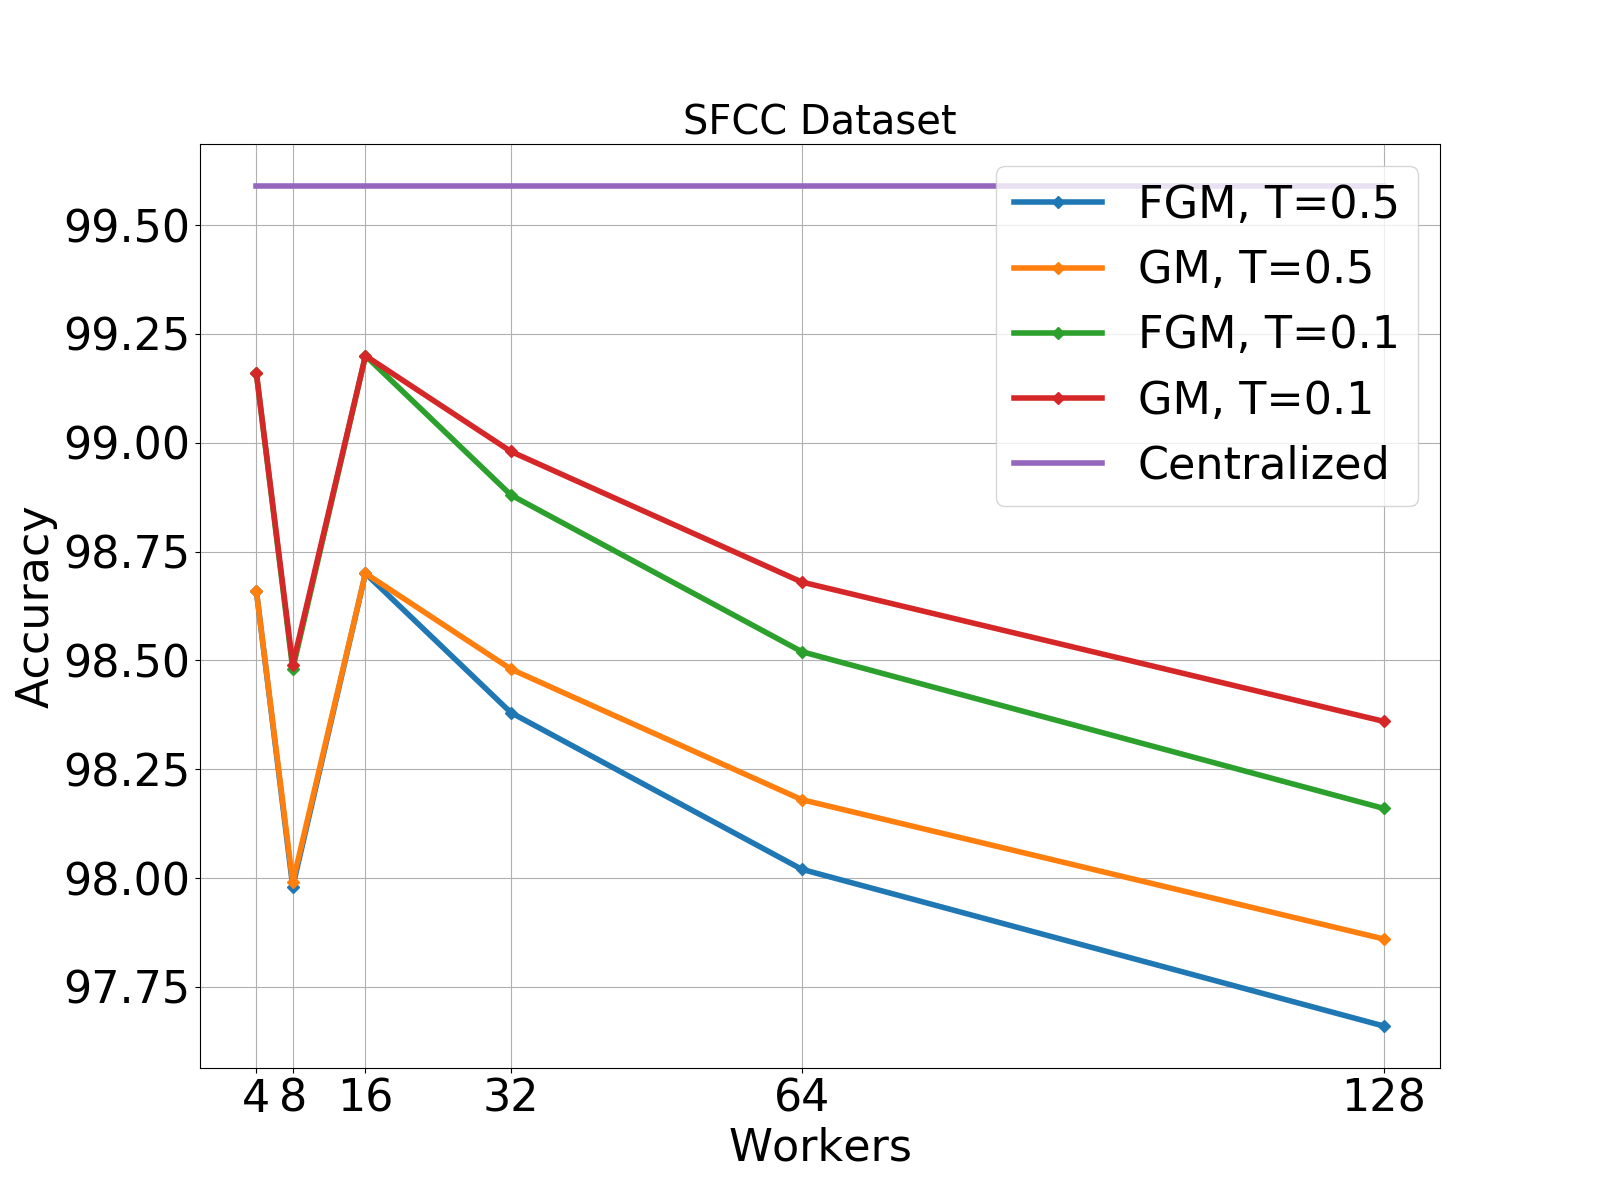
\includegraphics[width=\textwidth]{./images/results/sfc-plots/exp_Fig_3_1_b.png}
        \caption{}
    \end{subfigure}
    \begin{subfigure}[b]{0.48\textwidth}
        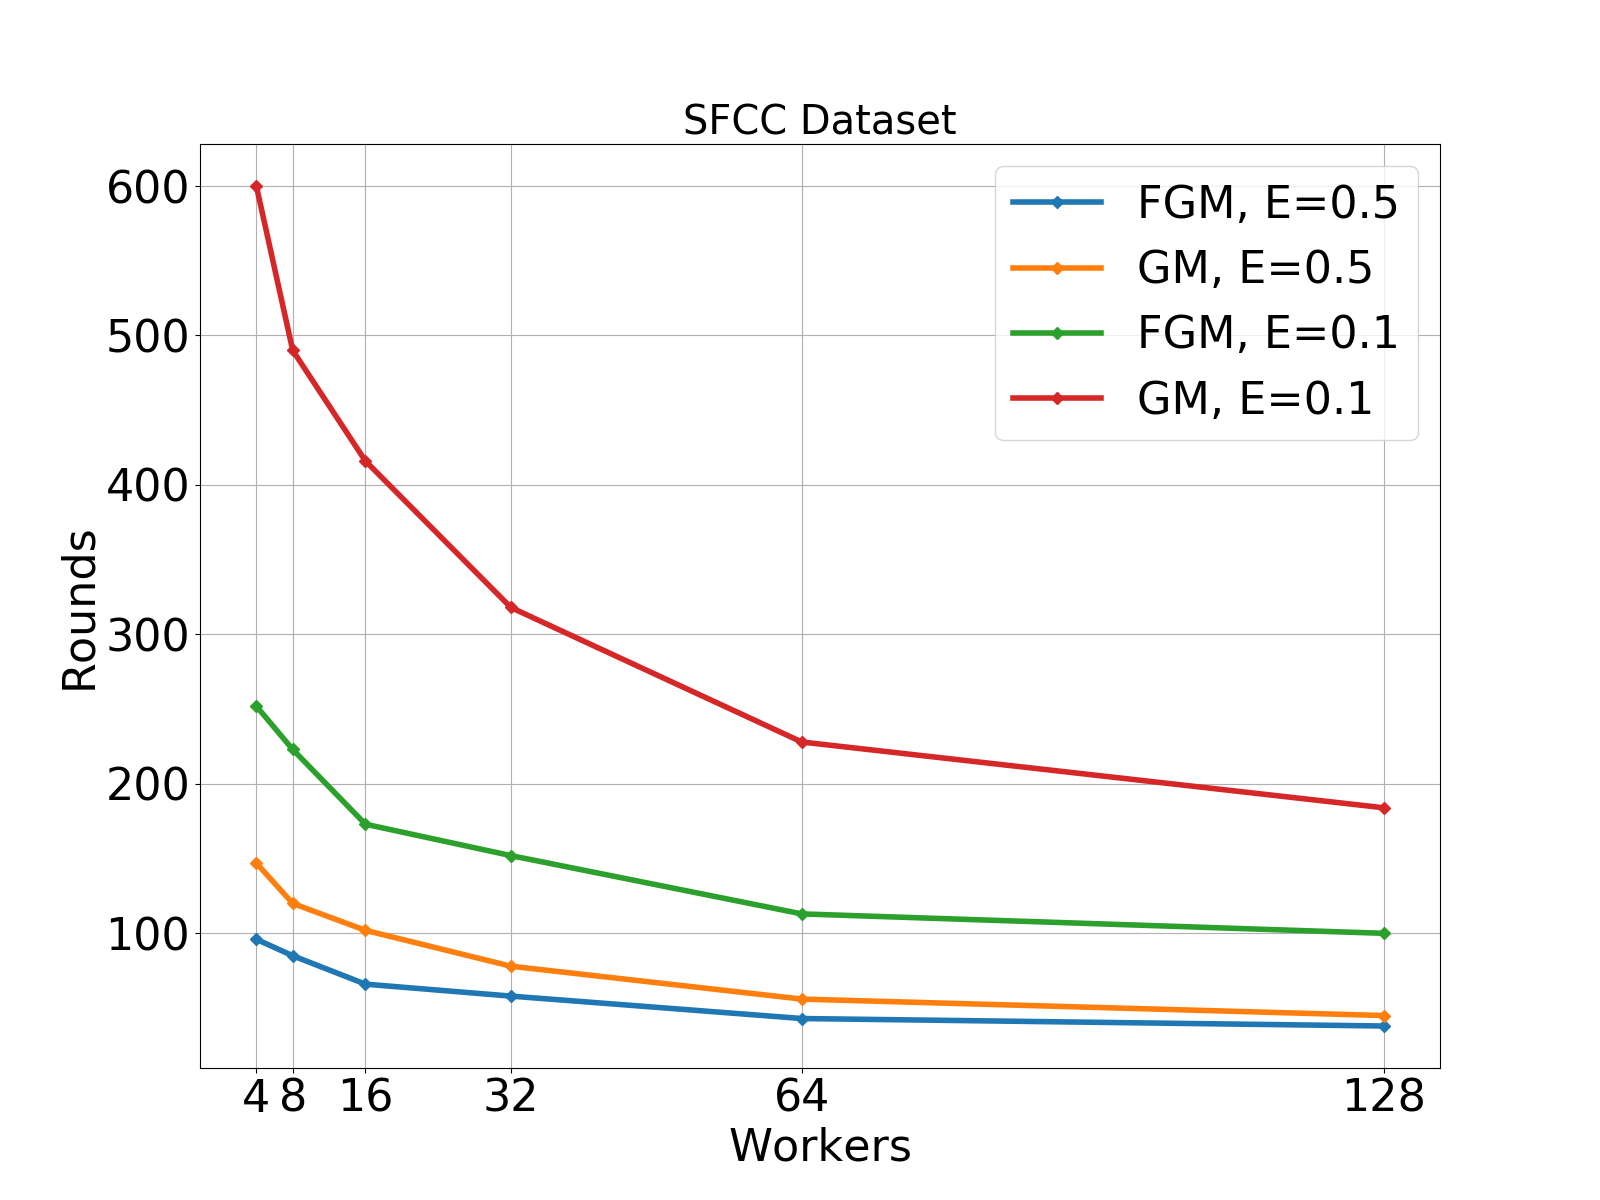
\includegraphics[width=\textwidth]{./images/results/sfc-plots/exp_Fig_3_2_b.png}
        \caption{}
    \end{subfigure}
    \begin{subfigure}[b]{0.50\textwidth}
        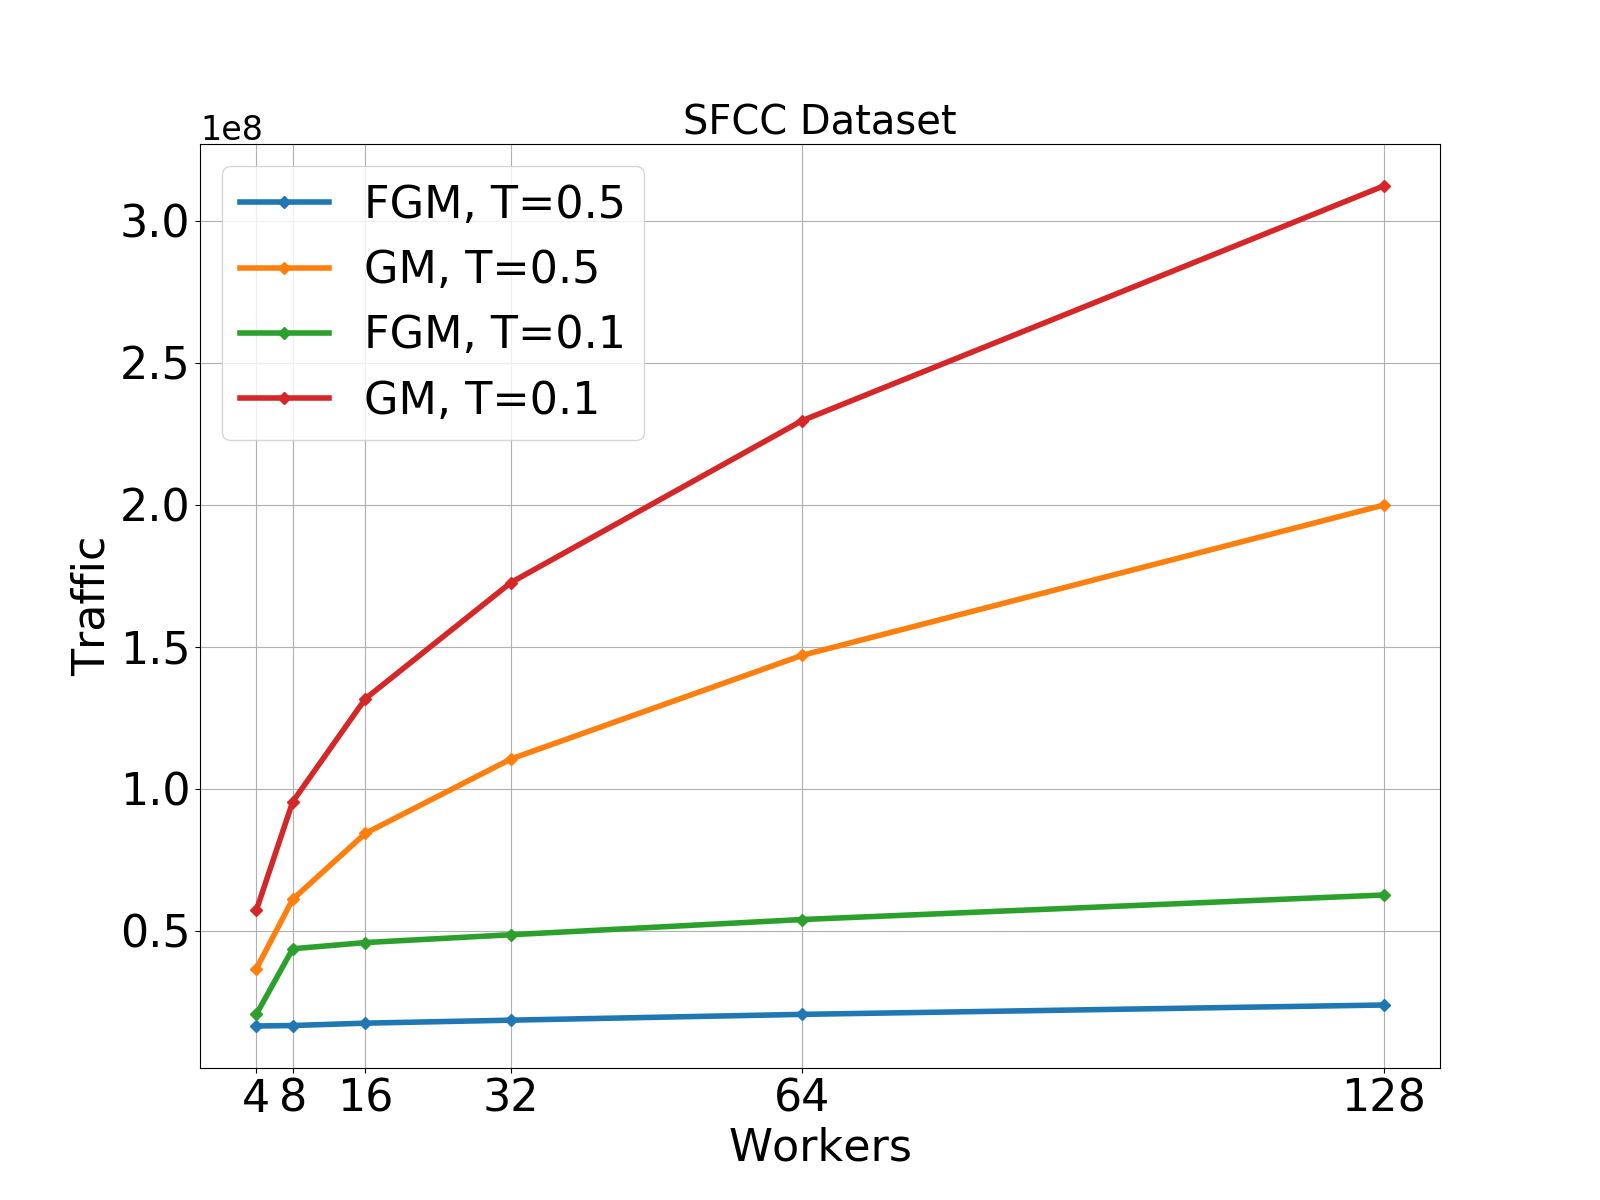
\includegraphics[width=\textwidth]{./images/results/sfc-plots/exp_Fig_3_3_b.png}
        \caption{}
    \end{subfigure}
    \caption{}
    \label{fig:sfcc_3_b}
\end{figure}

\newpage

\subsection{Safe functions comparison}\label{subsec:safe-functions-comparison}

In the second part of this work, I wanted to make a comparison between the two safe functions.
Michael Kamp used in his work the simple norm (Eq.~\ref{eq:equation33}) as his safe function.
I used the spherical cap (Eq.~\ref{eq:equation36}).
So, it remains to compare these functions to each other, to be able to decide which is the best for distributed Deep Learning.
For the sake of brevity, I define the simple norm safe function as '\emph{SF1}' and the spherical cap safe function as '\emph{SF2}'.

\begin{figure}[H]
    \centering
    \begin{subfigure}[b]{0.48\textwidth}
        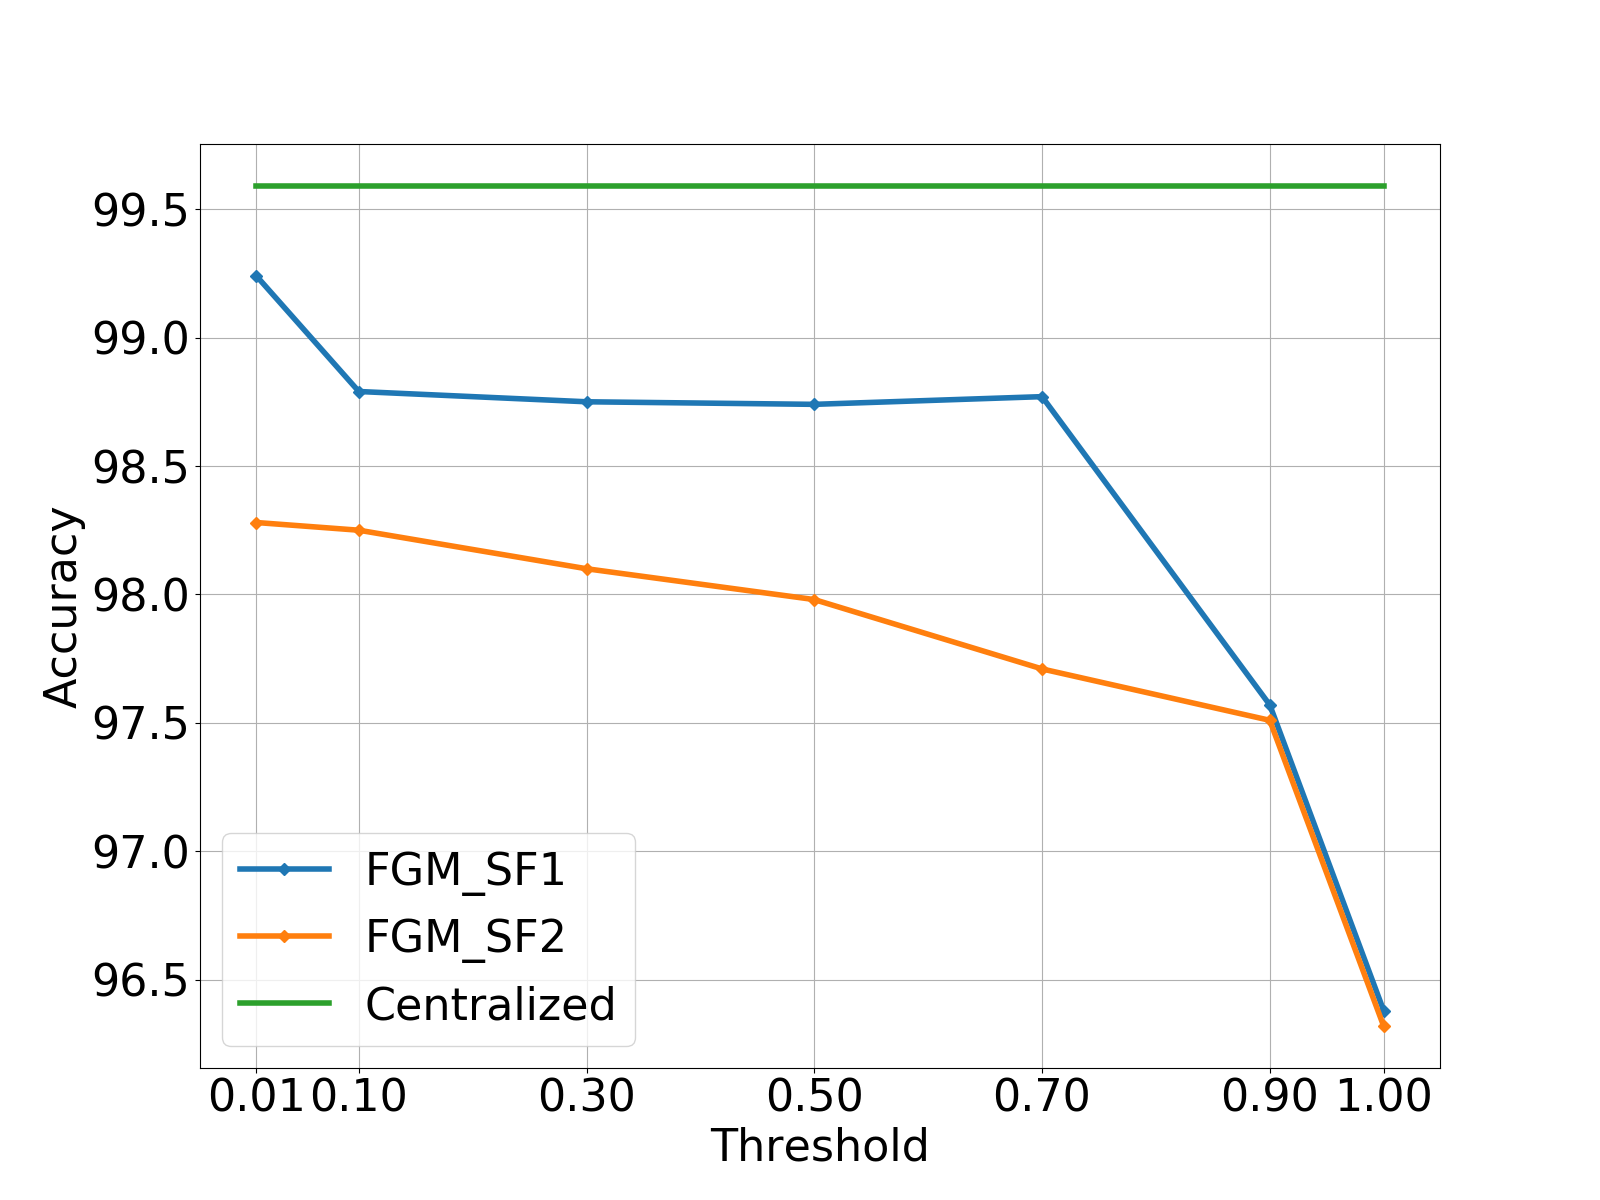
\includegraphics[width=\textwidth]{./images/results/sf-comp/exp_Fig_1_1.png}
        \caption{}
    \end{subfigure}
    \begin{subfigure}[b]{0.48\textwidth}
        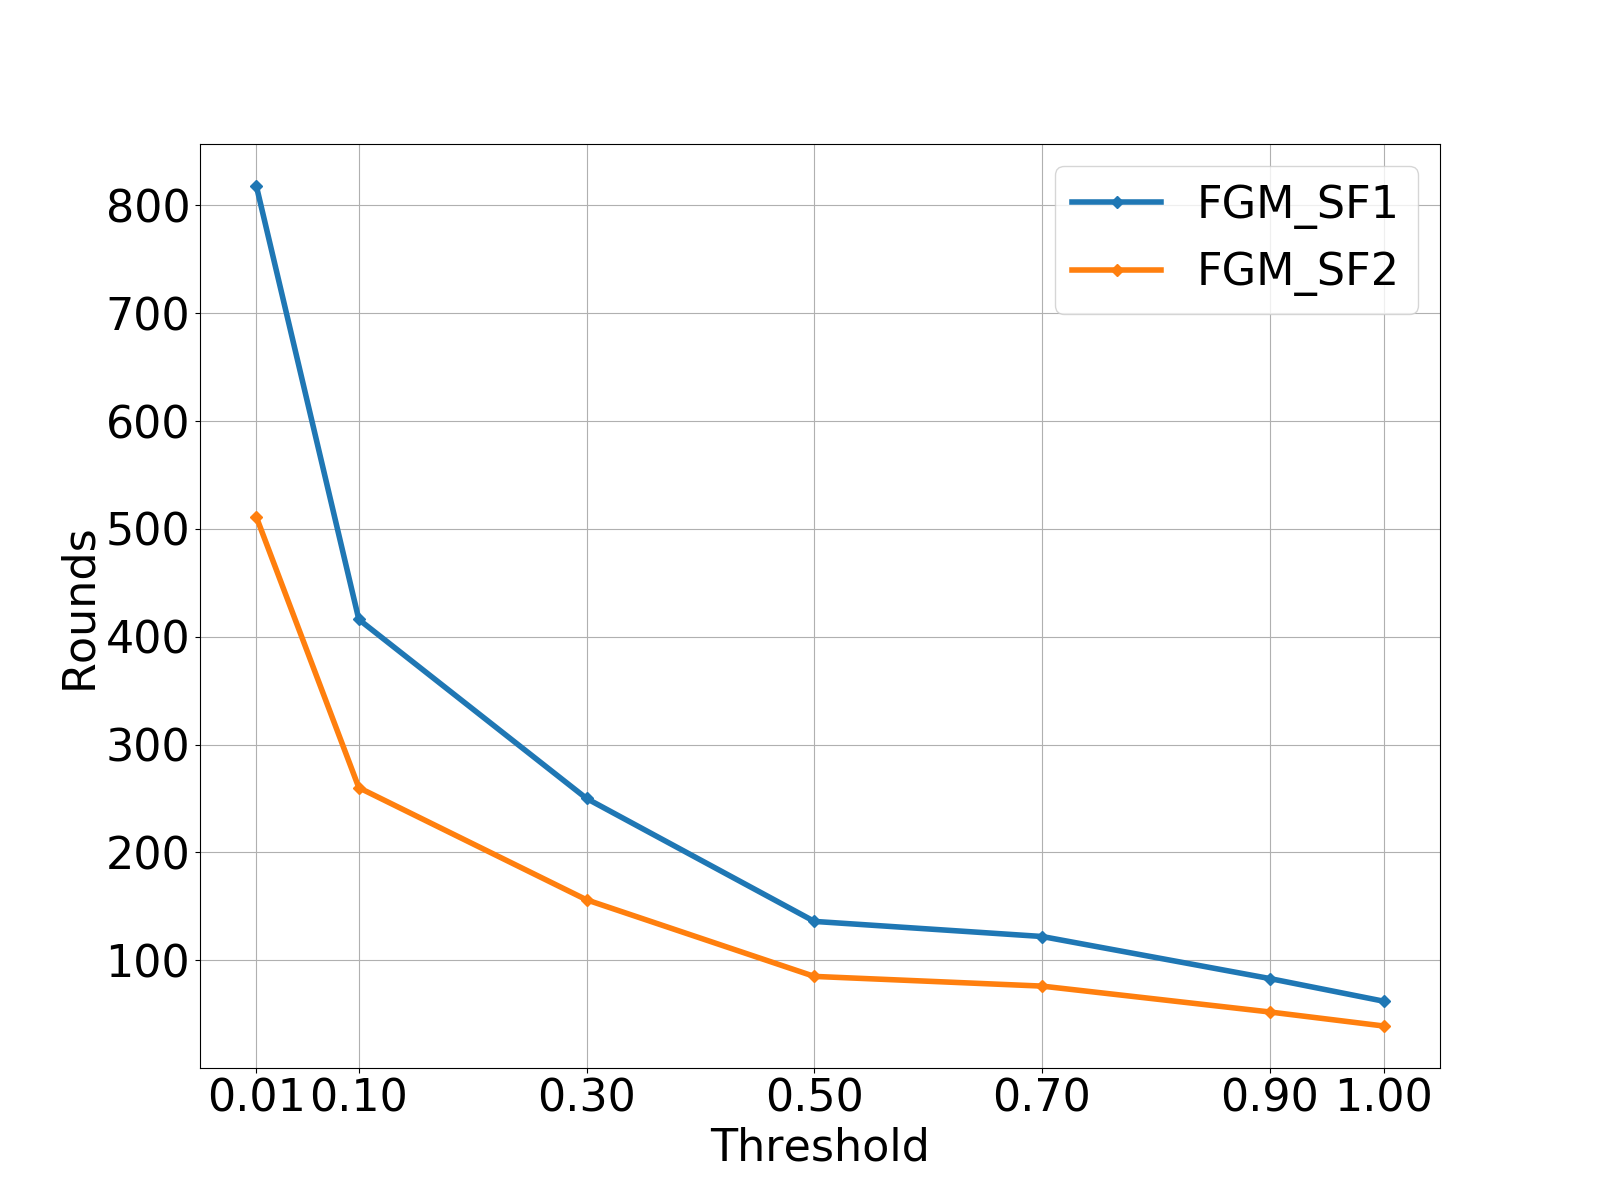
\includegraphics[width=\textwidth]{./images/results/sf-comp/exp_Fig_1_2.png}
        \caption{}
    \end{subfigure}
    \begin{subfigure}[b]{0.50\textwidth}
        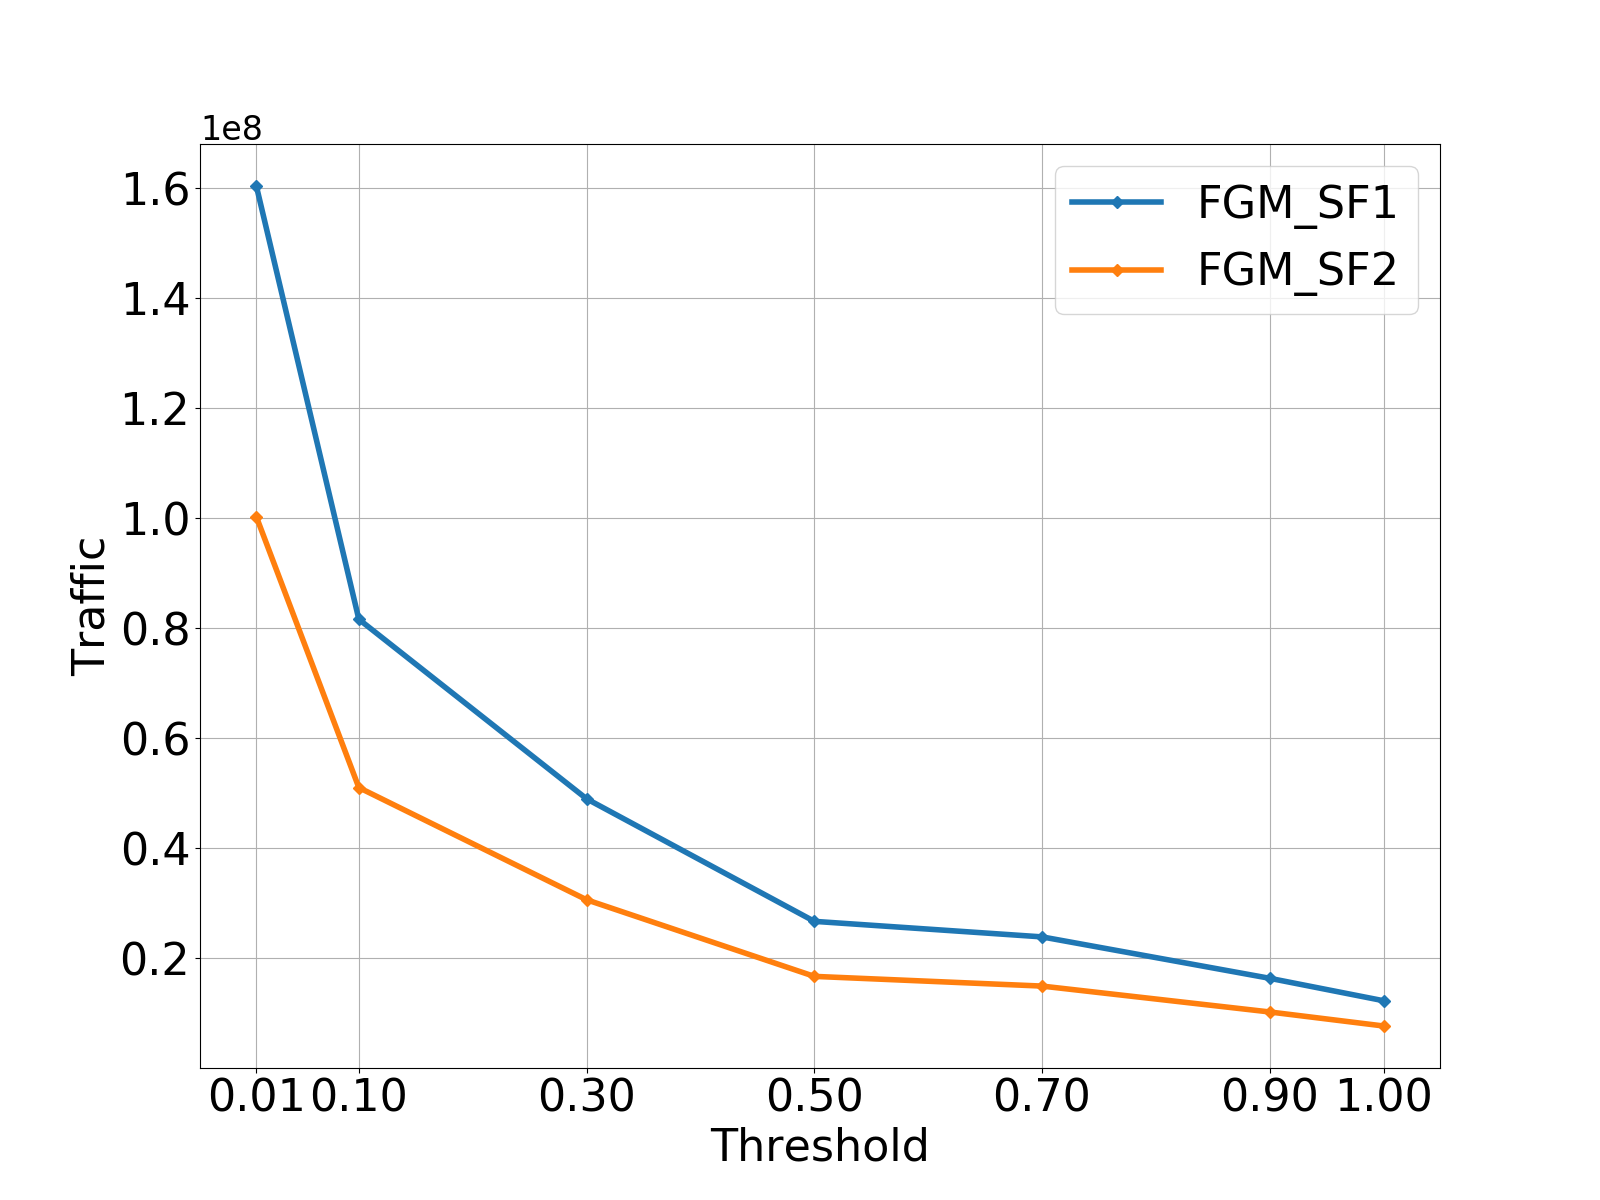
\includegraphics[width=\textwidth]{./images/results/sf-comp/exp_Fig_1_3.png}
        \caption{}
    \end{subfigure}
    \caption{}
    \label{fig:sf_1}
\end{figure}

When threshold is greater than $0.9$ (Fig.~\ref{fig:sf_1} A), we see that both functions achieve the same accuracy.
SF1 is more wasteful due to its geometry, so achieves more accuracy.
This accuracy is approx up to $1\%$.
For this reason, the number of rounds are more than the SF2 (Fig.~\ref{fig:sf_1} B).
Especially, with threshold $< 0.1$, the difference is the maximum between the two functions.
In figure~\ref{fig:sf_1} C, both curves follows the same direction as the above, which is reasonable.
In this case, rounds and traffic are proportional amounts.

\begin{figure}[H]
    \centering
    \begin{subfigure}[b]{0.48\textwidth}
        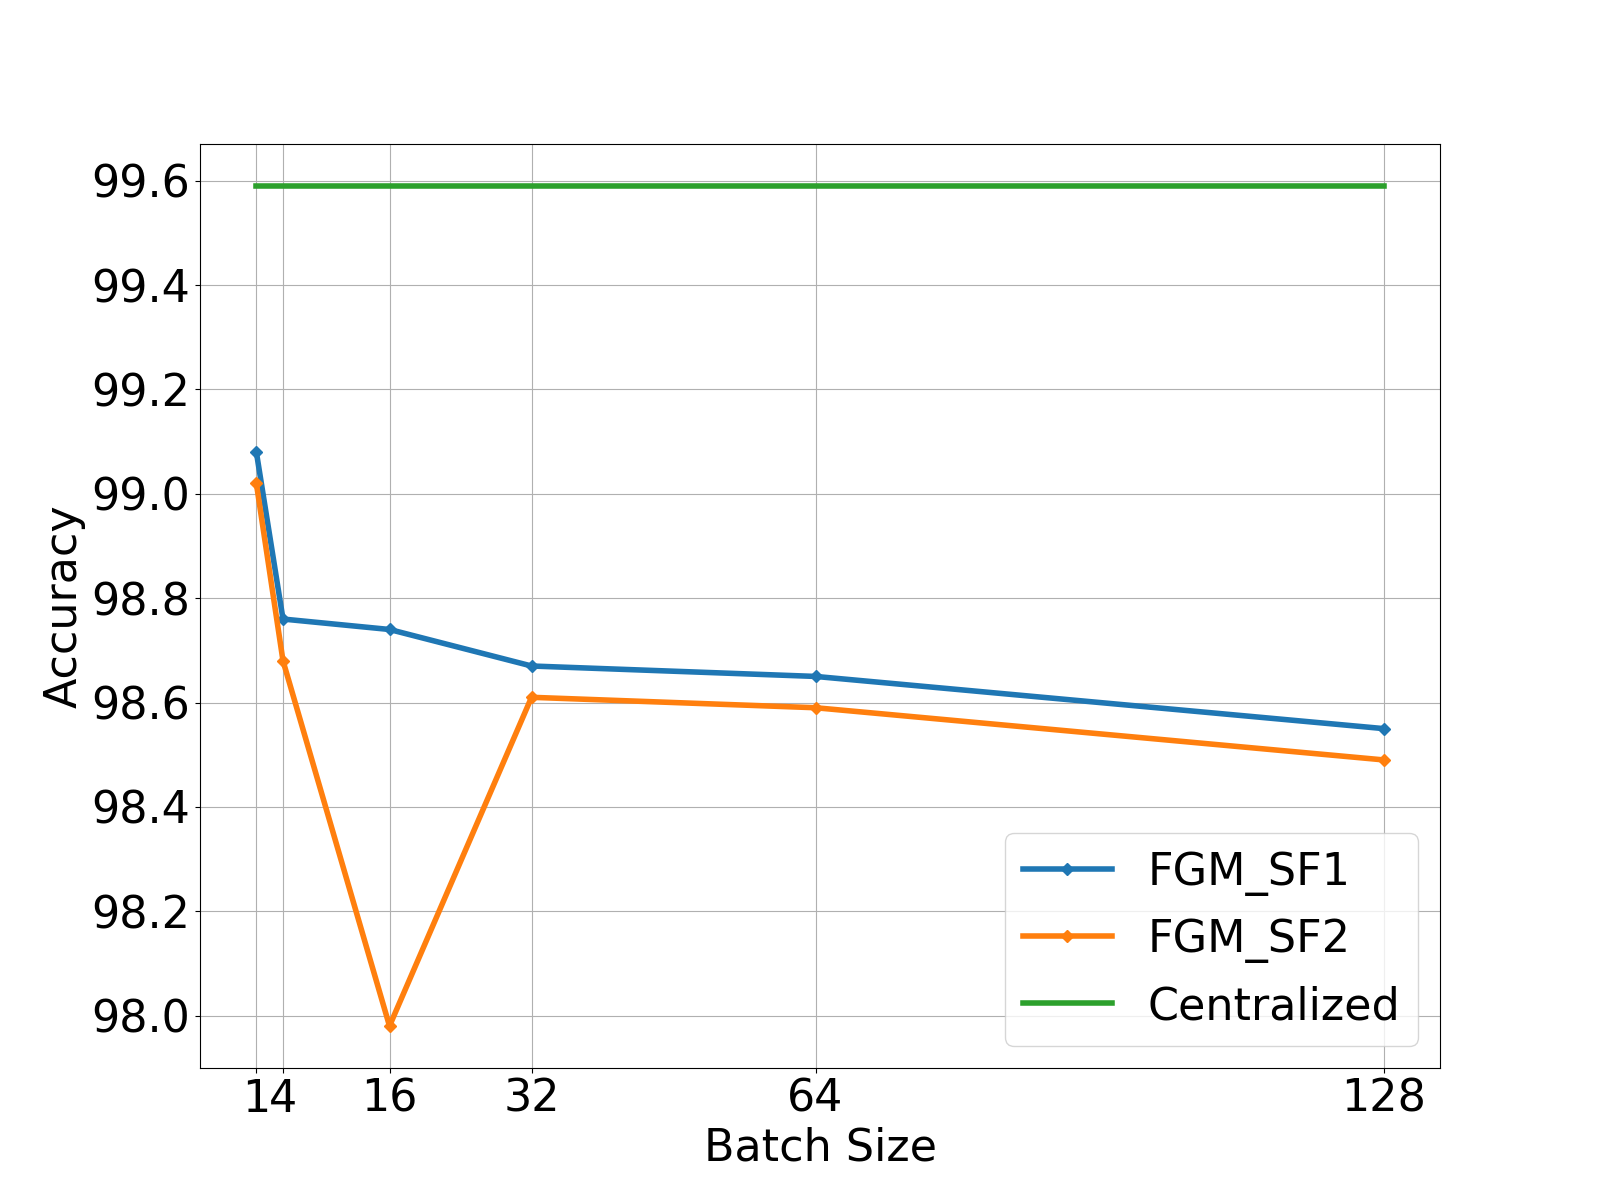
\includegraphics[width=\textwidth]{./images/results/sf-comp/exp_Fig_2_1.png}
        \caption{}
    \end{subfigure}
    \begin{subfigure}[b]{0.48\textwidth}
        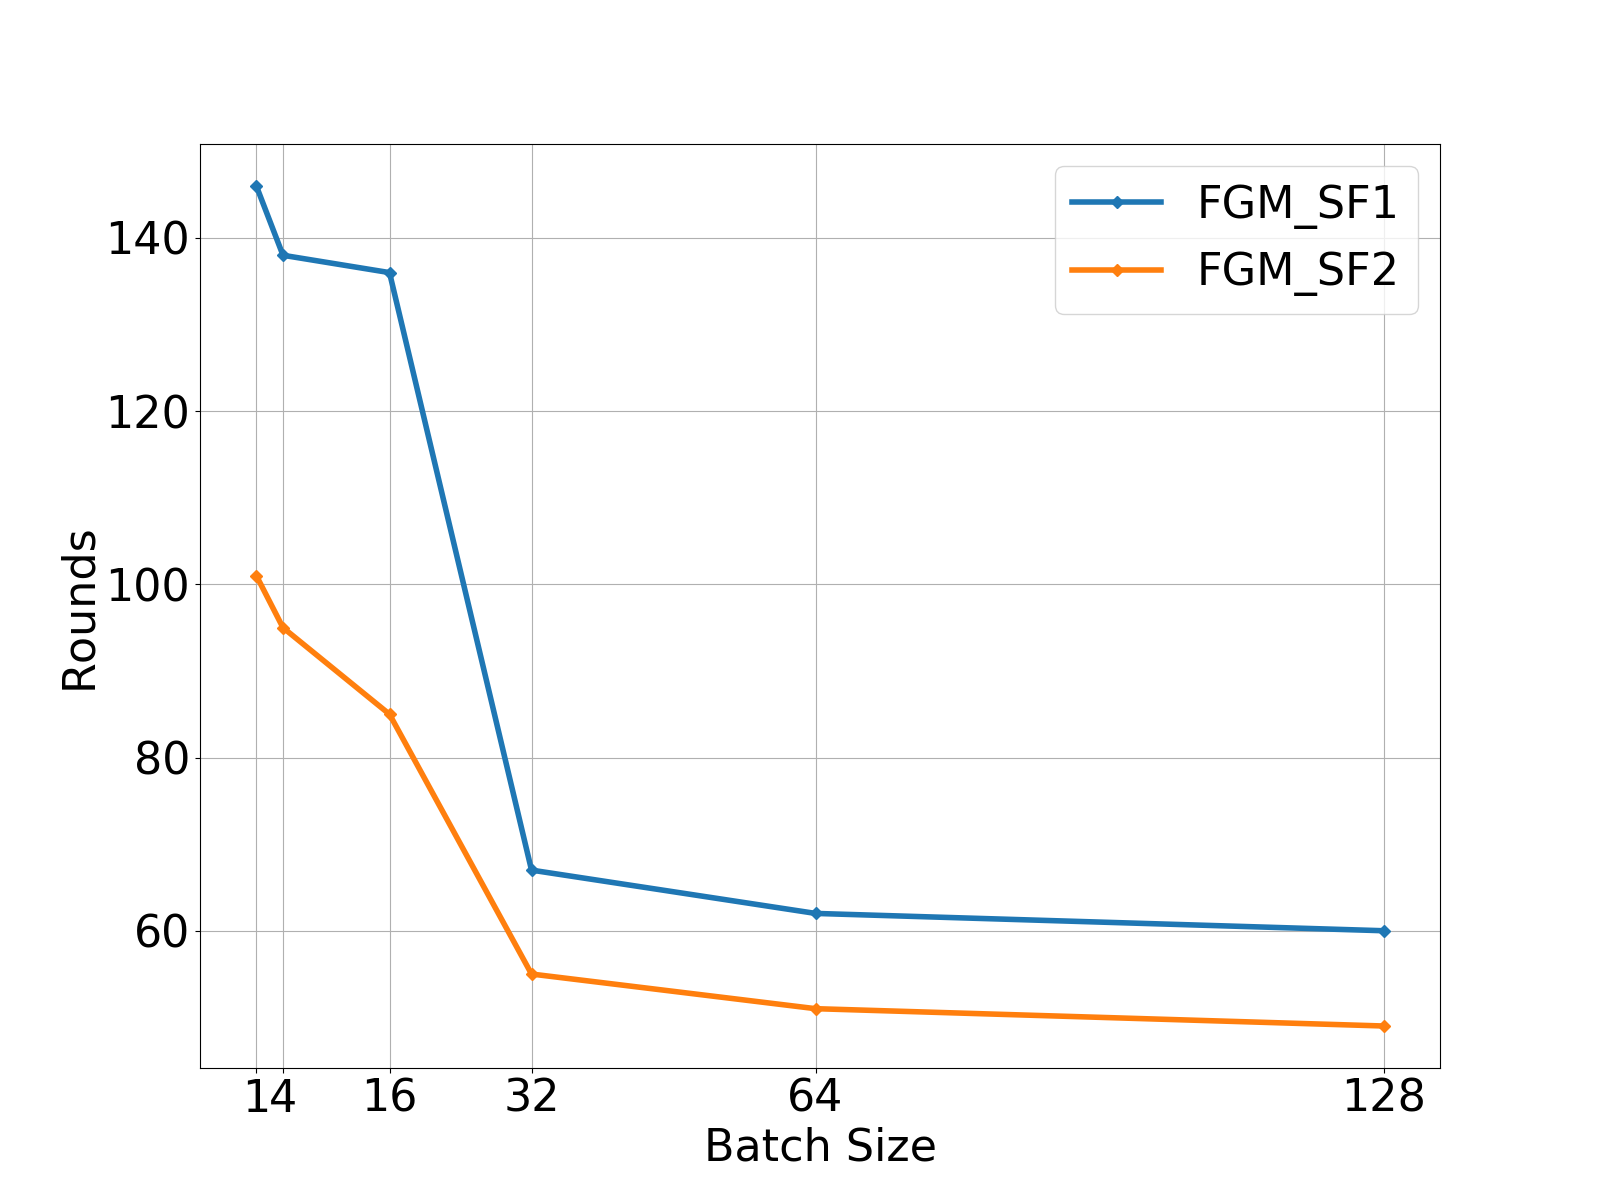
\includegraphics[width=\textwidth]{./images/results/sf-comp/exp_Fig_2_2.png}
        \caption{}
    \end{subfigure}
    \begin{subfigure}[b]{0.50\textwidth}
        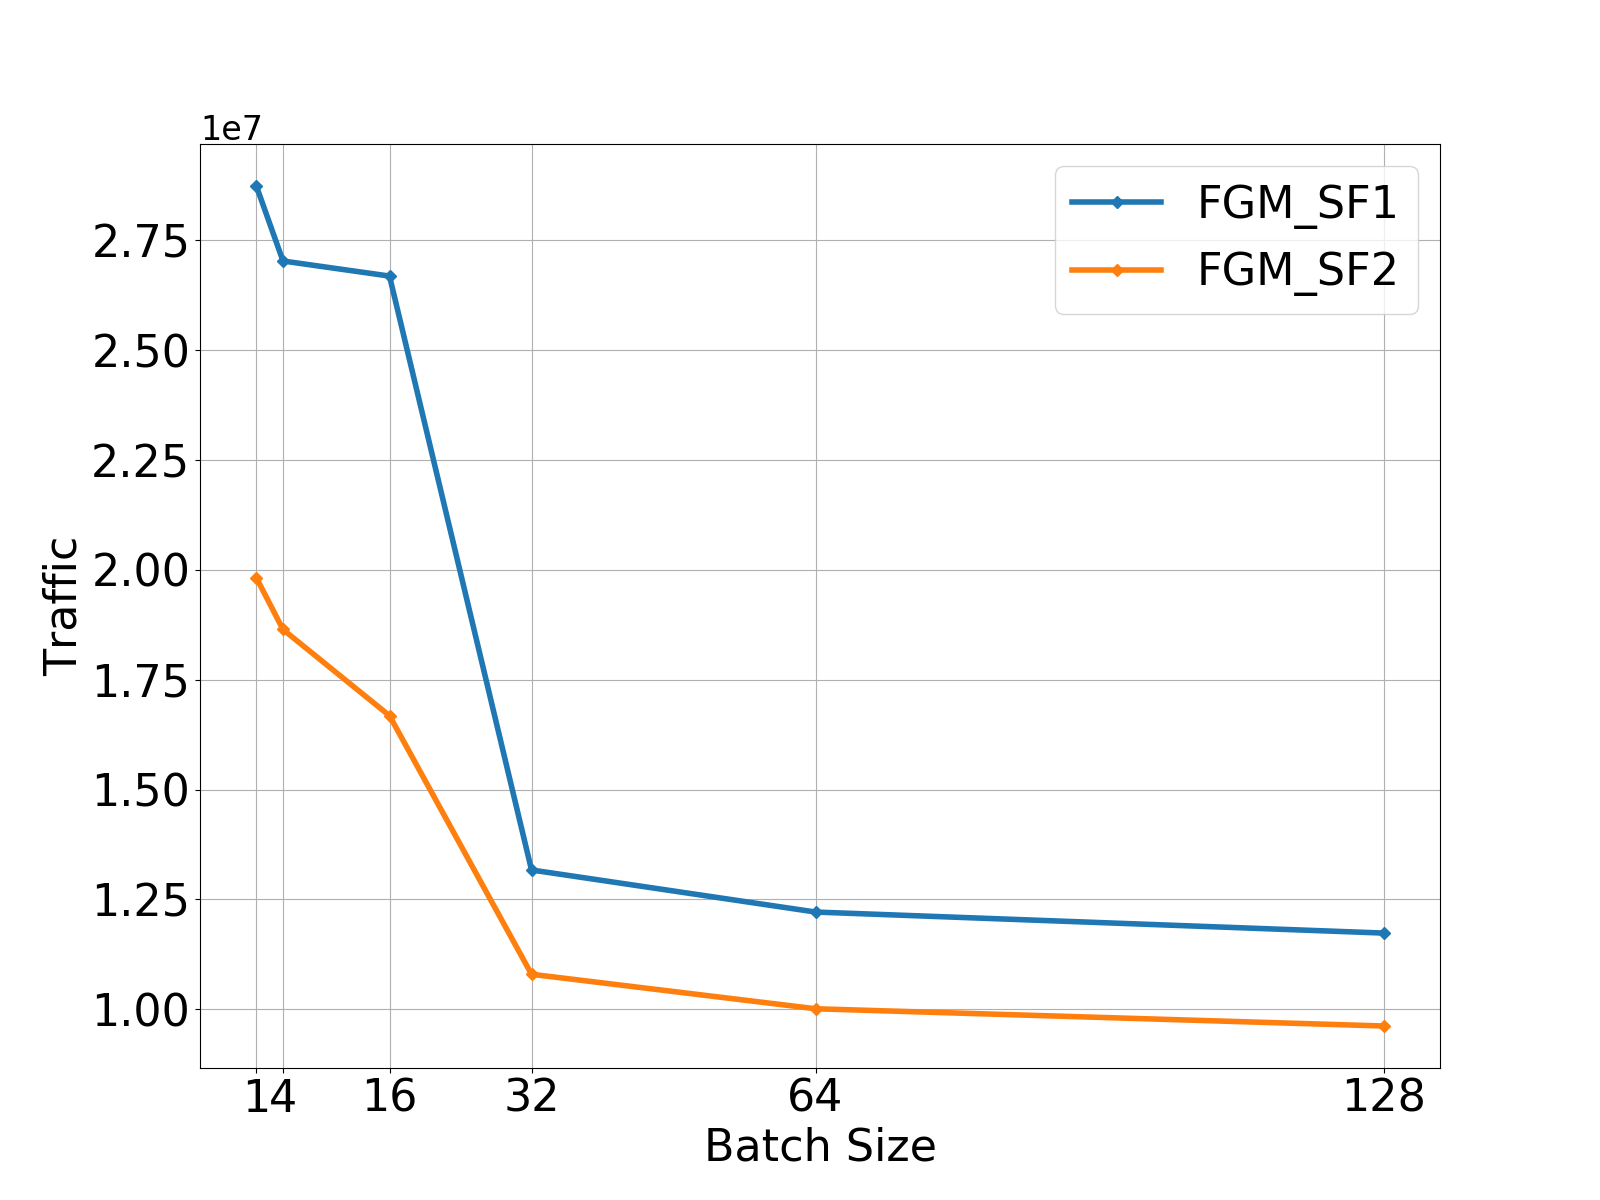
\includegraphics[width=\textwidth]{./images/results/sf-comp/exp_Fig_2_3.png}
        \caption{}
    \end{subfigure}
    \caption{}
    \label{fig:sf_2}
\end{figure}

Here we have another one outlier (Fig.~\ref{fig:sf_2} A).
Both safe functions have approximately the same accuracy when the batch size changes.
In Fig.~\ref{fig:sf_2} B, we can detect that for small batch sizes, the functions reach up to $50\%$ percentage change.
In the same way (Fig.~\ref{fig:sf_2} C), SF2 is better up to $42\%$.

\begin{figure}[H]
    \centering
    \begin{subfigure}[b]{0.48\textwidth}
        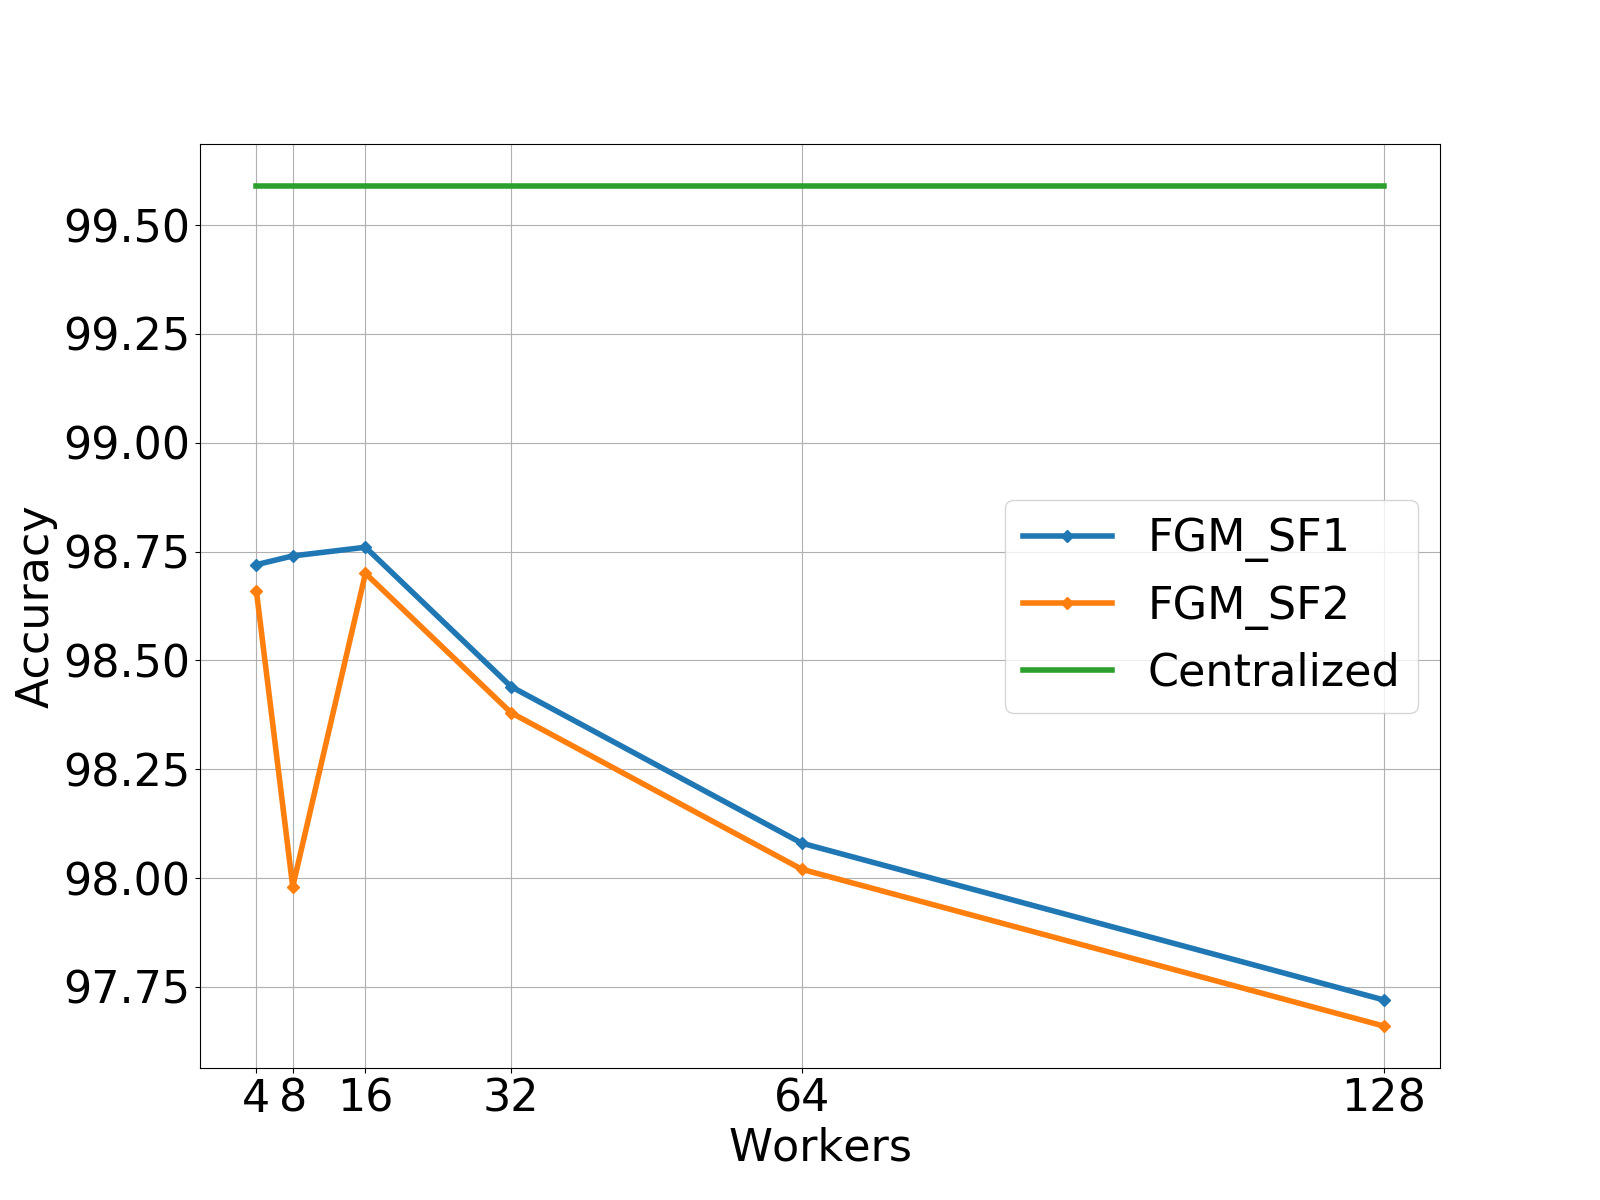
\includegraphics[width=\textwidth]{./images/results/sf-comp/exp_Fig_3_1.png}
        \caption{}
    \end{subfigure}
    \begin{subfigure}[b]{0.48\textwidth}
        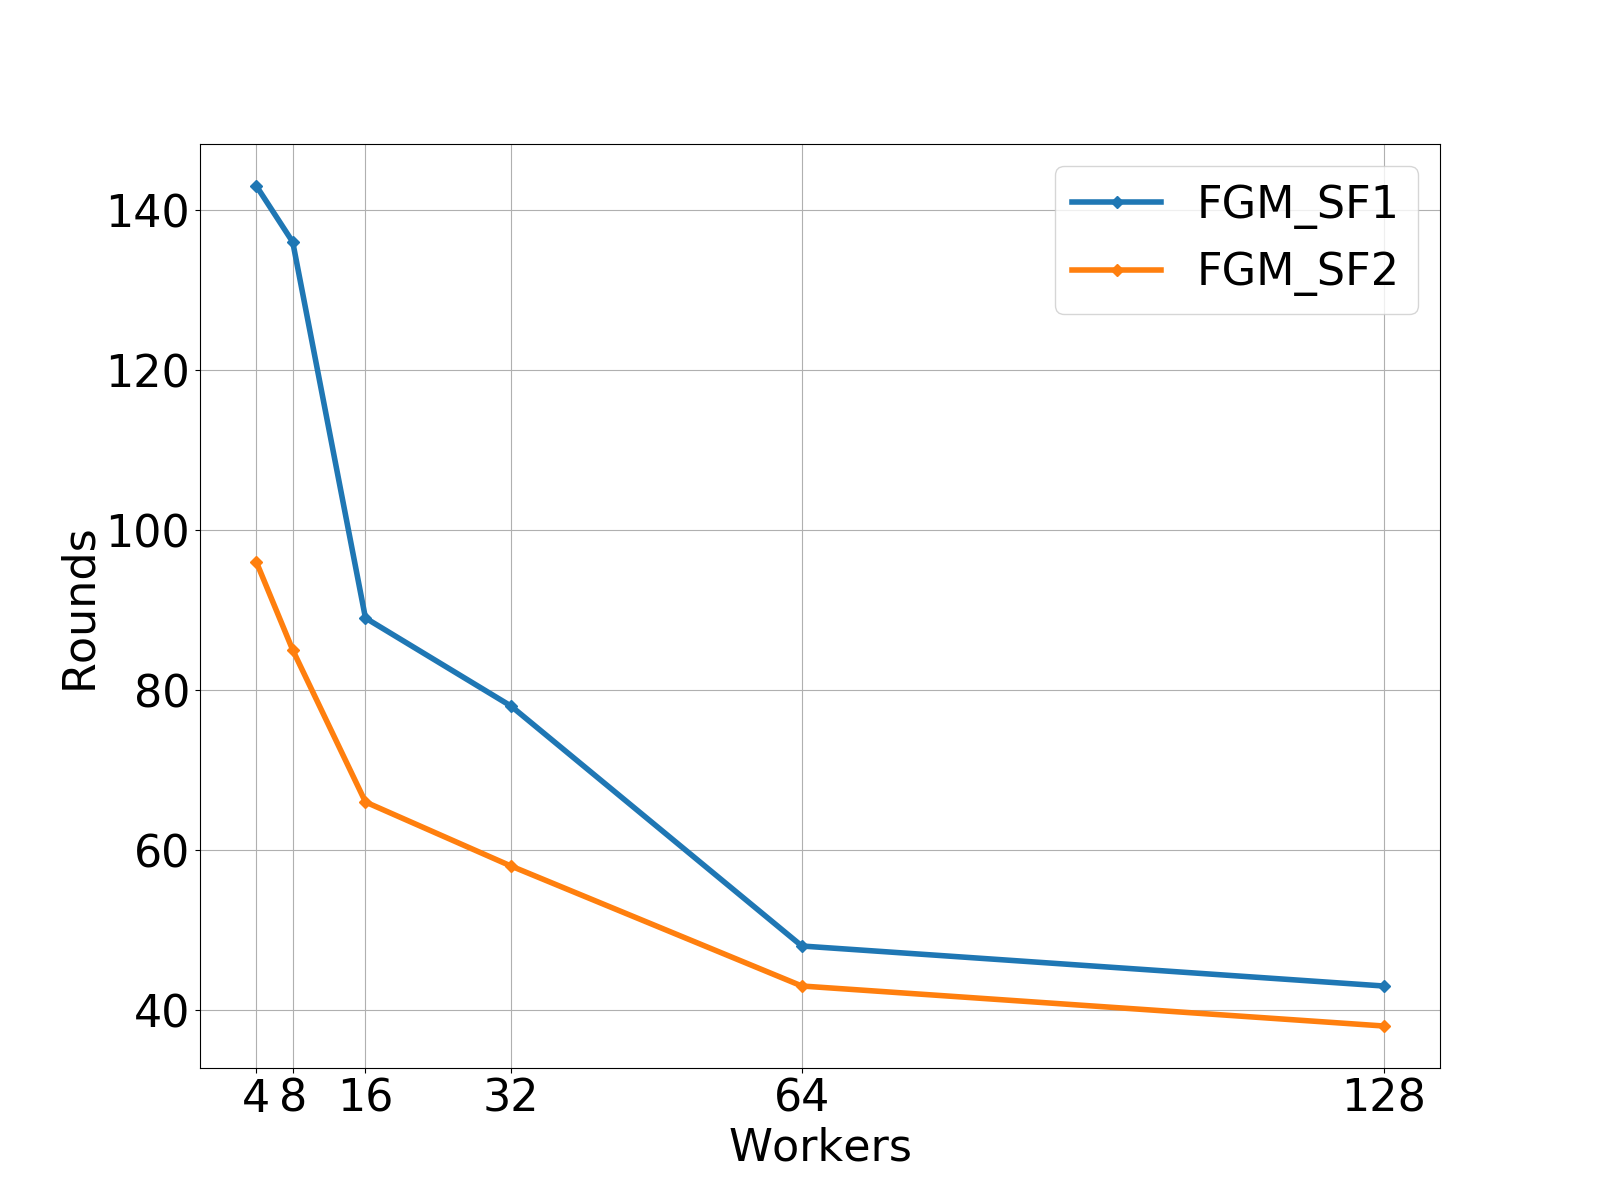
\includegraphics[width=\textwidth]{./images/results/sf-comp/exp_Fig_3_2.png}
        \caption{}
    \end{subfigure}
    \begin{subfigure}[b]{0.50\textwidth}
        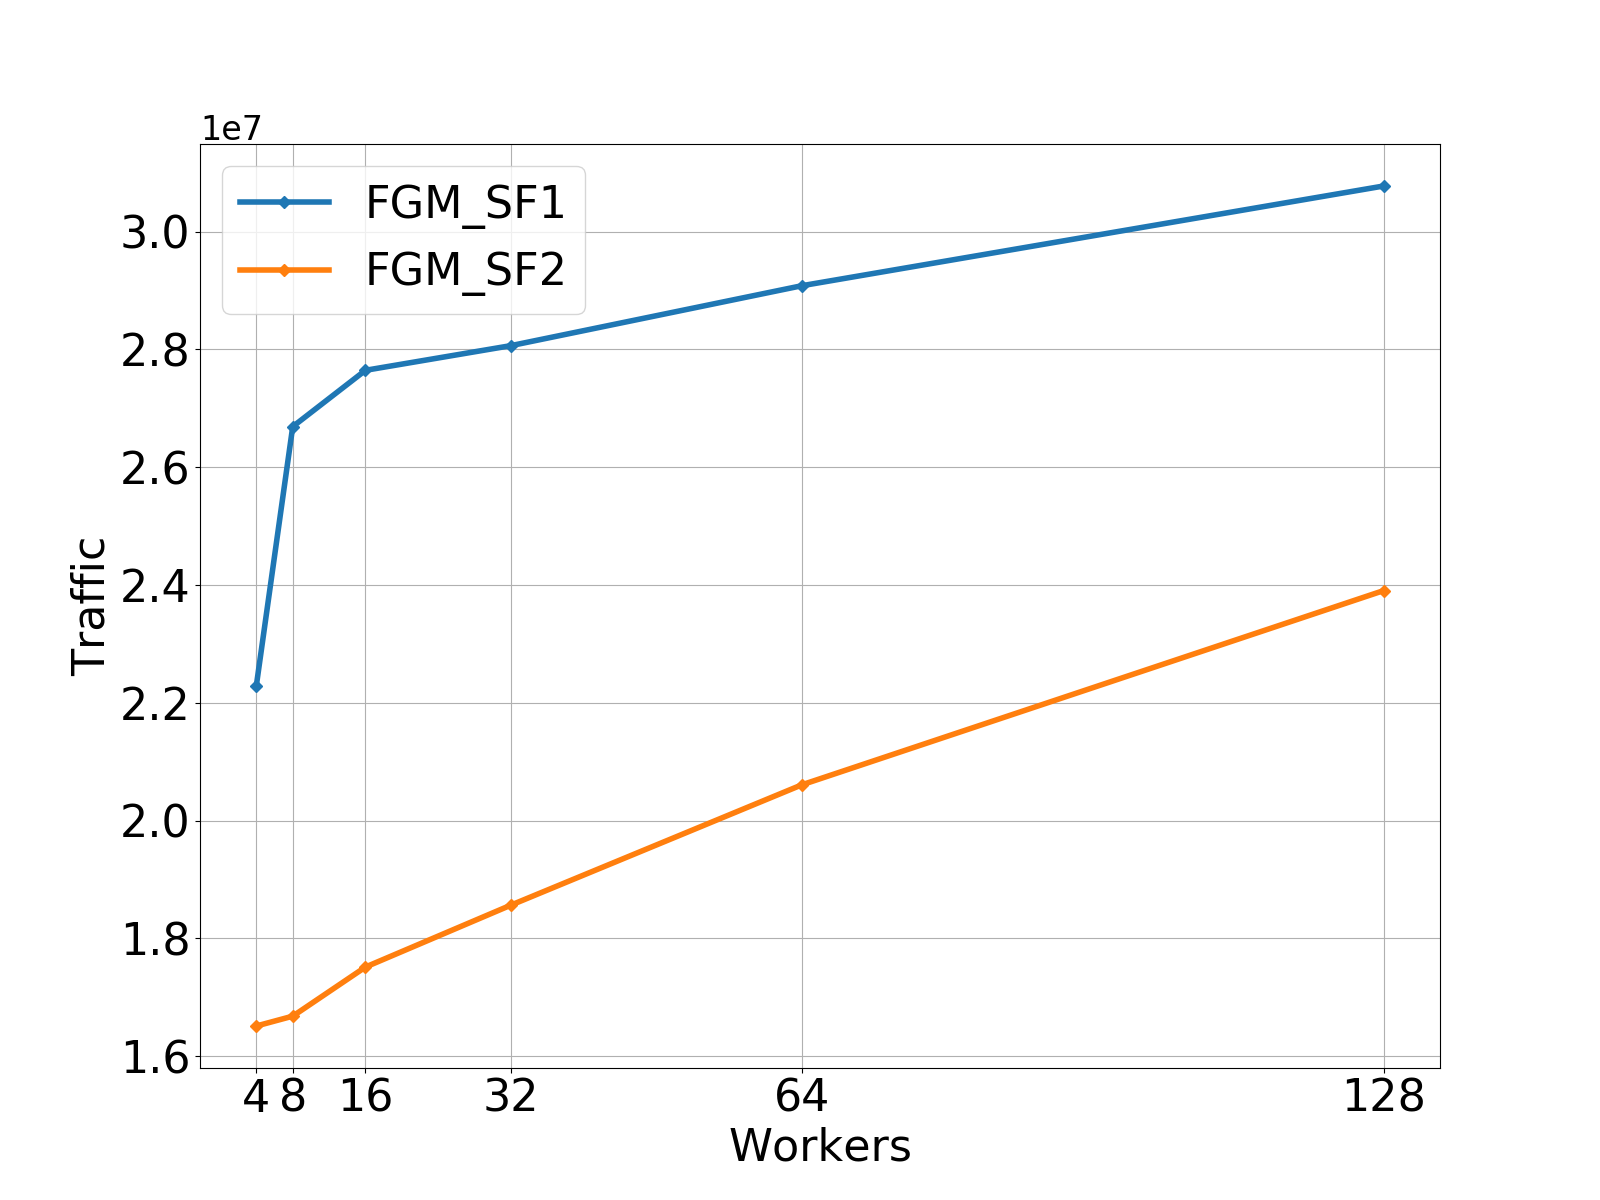
\includegraphics[width=\textwidth]{./images/results/sf-comp/exp_Fig_3_3.png}
        \caption{}
    \end{subfigure}
    \caption{}
    \label{fig:sf_3}
\end{figure}

Both accuracy and number of rounds on the number of workers (Fig.~\ref{fig:sf_3} A, B) follow the expected direction.
While the network is getting bigger (Fig.~\ref{fig:sf_3} C), SF2 is more efficient by up to $56\%$.
The maximum difference is noted when the workers are $8$.
After that, the change is less about $10\%$ compared to the maximum difference.
